%% ============================================================
%%  Threshold Bunching in Published Finance Research:
%%  Pre-Publication Evidence from Government-Intervention Studies
%%
%%  Target: Journal of Corporate Finance
%%
%%  Compile: pdflatex main.tex
%%           bibtex main
%%           pdflatex main.tex
%%           pdflatex main.tex
%% ============================================================

\documentclass[12pt]{article}

%% ---- Packages -----------------------------------------------
\usepackage[margin=1.25in]{geometry}
\usepackage{setspace}
\doublespacing
\usepackage{amsmath,amssymb}
\usepackage{booktabs}
\usepackage{tabularx}
\usepackage{longtable}
\usepackage{graphicx}
\usepackage{float}
\usepackage[dvipsnames]{xcolor}
\usepackage{hyperref}
\hypersetup{
  colorlinks=true,
  linkcolor=black,
  citecolor=black,
  urlcolor=NavyBlue
}
\usepackage{natbib}
\bibpunct{(}{)}{;}{a}{,}{,}
\usepackage{microtype}
\usepackage{caption}
\captionsetup[table]{
  labelfont={bf},
  textfont={normalsize},
  labelsep=period,
  justification=raggedright,
  singlelinecheck=false,
  skip=6pt
}
\captionsetup[figure]{font=small,labelfont=bf,labelsep=period}
\renewcommand{\tablename}{Table}
\renewcommand{\figurename}{Figure}
\usepackage{threeparttable}
\usepackage{multirow}
\usepackage{rotating}
\usepackage{pdflscape}
\usepackage{url}
\usepackage{enumitem}
\usepackage{footmisc}
\usepackage{titlesec}
\usepackage{titletoc}

%% ---- JCF-style section/subsection formatting ----------------
%% Sections: Arabic numeral, bold, flush left, title case
\titleformat{\section}
  {\normalfont\large\bfseries}
  {\arabic{section}.}{0.5em}{}
\titlespacing*{\section}{0pt}{18pt}{8pt}

%% Subsections: 2.1 dot notation, bold, flush left
\titleformat{\subsection}
  {\normalfont\normalsize\bfseries}
  {\arabic{section}.\arabic{subsection}}{0.5em}{}
\titlespacing*{\subsection}{0pt}{12pt}{4pt}

%% Sub-subsections: normal size italic
\titleformat{\subsubsection}
  {\normalfont\normalsize\itshape}
  {}{0em}{}
\titlespacing*{\subsubsection}{0pt}{8pt}{3pt}

%% Arabic table and figure numbering
\renewcommand{\thetable}{\arabic{table}}
\renewcommand{\thefigure}{\arabic{figure}}

%% References heading
\renewcommand{\refname}{References}

%% ---- Custom commands ----------------------------------------
\newcommand{\JF}{\textit{Journal of Finance}}
\newcommand{\RFS}{\textit{Review of Financial Studies}}
\newcommand{\JFE}{\textit{Journal of Financial Economics}}
\DeclareMathOperator{\Prob}{Pr}

%% ---- Title block --------------------------------------------
\title{Do Finance Journals Sort on Policy Conclusions?%
}

\author{Emre Kuvvet%
        \thanks{Department of Finance, Nova Southeastern University. E-mail: ekuvvet@nova.edu.}}

\date{\today}

\setlength{\emergencystretch}{3em}   % allow slightly looser lines to prevent overflow

\begin{document}
\hypersetup{pageanchor=false}
\maketitle
\thispagestyle{empty}

\vspace{4pt}
\begin{center}{\normalsize\bf ABSTRACT}\end{center}
\begin{singlespace}
\noindent\small
We study whether top finance journals favor certain policy conclusions.
Using 121 published articles in the \JF{}, \RFS{}, and \JFE{} alongside
125 NBER working papers on government intervention in financial markets
(2000--2024), we find that journals do not sort on finding direction.
Whether a paper concludes that a regulation is beneficial, harmful, or
inconsequential, it reaches a top journal at roughly the same rate, about
46 percent.  The strongest predictor of publication is research design:
papers using quasi-experimental methods are about 18 percentage points
more likely to be published, regardless of what they find.  We also find
that published papers show modest threshold bunching in supplementary test
statistics but not in their main regression tables, suggesting that any
specification searching is concentrated at the margins of the paper rather
than in its core results.
\end{singlespace}
\vspace{4pt}
\noindent\small\textit{JEL classification:} G18, G28, C80, B40.

\noindent\small\textit{Keywords:} Publication bias; Government intervention; Finance journals; Selective reporting; Regulatory finance; p-hacking

\clearpage
\hypersetup{pageanchor=true}
\setcounter{page}{1}

%% ============================================================
\section{Introduction}
\label{sec:intro}
%% ============================================================

Academic research on government intervention in financial markets occupies a
privileged position in public policy.  The Federal Reserve Board, the
Securities and Exchange Commission, and the Basel Committee on Banking
Supervision routinely incorporate peer-reviewed finance research into
regulatory impact assessments, rule-makings, and policy speeches.  The
Dodd-Frank Wall Street Reform and Consumer Protection Act alone generated an
estimated 400 new regulatory mandates, many of which were designed in explicit
reference to academic evidence on the effects of capital requirements,
disclosure rules, and consumer financial protection.  The credibility of this
evidence base is therefore a first-order policy question: if the academic record
systematically misrepresents which interventions have measurable effects---and
which do not---regulators face a distorted picture that can generate
welfare-reducing policy choices.

Publication bias offers a mechanism by which such distortion arises without any
deliberate misconduct.  When researchers are reluctant to write up null results,
when journals are more likely to accept papers with statistically significant
findings, or when both effects operate simultaneously, the published literature
understates the true prevalence of null or inconclusive evidence
\citep{Franco2014}.  In a domain such as government intervention research,
where policy decisions depend on whether a regulation has a measurable causal
effect, suppression of null results generates the false impression that most
interventions work---or, more precisely, that most interventions have discernible
effects in one direction or the other.

Why might directional publication bias arise in the government-intervention
literature specifically?  Two theoretical channels operate in opposite
directions, making the sign of any bias an open empirical question.  A
\textit{pro-intervention channel} could arise if journals and readers favor
results that confirm a policy's stated objective (e.g., that capital
requirements reduce bank risk), both because positive results are more
actionable for regulators and because they more naturally confirm the prior
that motivated the policy.  An \textit{anti-intervention channel} could arise
if research that documents unintended costs or failures of regulation is more
surprising---and thus more publishable---than research confirming that a
policy works as intended.  Under either channel, the direction of sorting
would differ from significance bias (null vs.\ directional), which reflects a
simpler threshold between finding-something and finding-nothing.  This paper
is designed to detect both types.

This paper studies sorting patterns in a domain the existing literature has
not examined: the finance literature's treatment of government intervention.
Prior work on publication bias in finance has focused on the cross-section of
asset pricing anomalies, documenting that factor-zoo proliferation reflects
selection for high t-statistics \citep{Harvey2016,Hou2020,Jensen2023}.  A
parallel economics literature \citep{Brodeur2016,Andrews2019} infers bias from
the shape of published p-value distributions, finding excess mass just below
conventional significance thresholds.  Neither strand addresses the
policy-intervention literature, nor do they distinguish two conceptually
distinct forms of bias with different welfare implications.
\textit{Significance bias}---directional findings over-published relative to
null findings---makes every intervention appear detectable.
\textit{Directional bias}---pro-intervention findings over-published relative
to anti-intervention findings---additionally skews the regulatory record toward
a particular conclusion about the sign of policy effects.  We design our study
to test for both.

Our research design combines two complementary samples.  The
\textit{published paper} sample consists of all in-scope articles in the \JF{},
the \RFS{}, and the \JFE{} from 2000 to 2024.  The \textit{working paper}
sample is drawn from NBER working papers in five programs covering the dominant
share of academic finance research on government intervention: Corporate Finance,
Asset Pricing, Monetary Economics, Economic Fluctuations and Growth, and Public
Economics.  The key advantage of this design is that we observe findings from
papers that circulated \textit{before} potential journal publication, allowing a
direct two-corpus comparison rather than inferring the pre-publication
distribution from the shape of published p-values alone.

Because only 12\% of published papers are matched to a confirmed NBER counterpart, the two corpora are largely non-overlapping cross-sections rather than the same papers tracked through the editorial filter.  We therefore interpret all estimates as cross-sectional associations between paper characteristics and corpus membership, not as causal editorial-filter effects; the full identification discussion is in Section~\ref{subsec:limitations}.

We define a paper as in-scope if its primary research question concerns the
causal effect of a specific government law, regulation, or public policy on
financial markets, firms, or investors.  Identifying these papers across
nearly 40,000 documents required an automated approach: a keyword filter
followed by a large language model (LLM) classifier that reads each abstract
and assigns an in-scope judgment along with a directional code---positive
($+1$, the intervention was beneficial), negative ($-1$, harmful), or
null/mixed ($0$).

Our central result is that finding direction does not predict publication.
Papers concluding that a regulation helps, papers concluding it hurts, and
papers finding no significant effect all reach the three top journals at
essentially the same rate---around 46 percent.  This uniformity holds
unconditionally and survives every regression specification we estimate,
including controls for publication year, decade, team size, and research
design quality.  The complete absence of a direction premium holds for
positive findings, for negative findings, and when positive and negative
are pooled against null.

What does predict publication is how a paper was designed.  Papers using
quasi-experimental identification strategies---regression discontinuity
designs, instrumental variables, difference-in-differences, or event
studies---are roughly 18 percentage points more likely to appear in a top
journal than observational papers on the same policy questions.  This
methodological premium is the only statistically robust predictor we find;
finding direction adds nothing beyond it.  We interpret this cautiously:
the quasi-experimental indicator likely captures a bundle of correlated
quality attributes---author prestige, institutional resources, topic
fashionability---not identification strategy alone.

Within published papers, we find a secondary pattern.  Test statistics
bunch modestly just below the conventional 5 percent significance threshold,
but only in standalone statistics that appear primarily in supplementary and
robustness tables.  Primary regression tables---where both a coefficient and
a standard error are reported and can be independently verified---show no
bunching and are statistically indistinguishable from the corresponding NBER
working paper tables.  This distinction is informative: it suggests that
any selective reporting occurs at the margin of revision, in the choice of
which additional checks to highlight, rather than in the core empirical
results that define the paper's contribution.

This paper makes three contributions: it provides direct evidence that top finance journals do not sort government-intervention research by the direction of its conclusions; it documents that identification quality---not finding direction---is the dominant sorting criterion, with papers using credible causal designs substantially more likely to be published; and it introduces a validated LLM-assisted pipeline for classifying and direction-coding large paper corpora, with code and prompts publicly available.

The remainder of the paper proceeds as follows.
Section~\ref{sec:literature} reviews the related literature.
Section~\ref{sec:data} describes data construction and the classification
pipeline.  Section~\ref{sec:methods} presents the empirical strategy.
Section~\ref{sec:results} reports main results and economic magnitudes.
Section~\ref{sec:robustness} presents robustness checks.
Section~\ref{sec:discussion} discusses mechanisms, policy implications,
comparisons to other domains, and limitations.
Section~\ref{sec:conclusion} concludes.

%% ============================================================
\section{Related Literature}
\label{sec:literature}
%% ============================================================

This paper relates to three strands of research.  The first is the literature
on publication bias in economics and finance.  \citet{Brodeur2016} document
excess mass just below the 5\% significance threshold in the top economics
journals, consistent with selective reporting of marginally significant
specifications.  \citet{Franco2014} show, using NSF-funded pre-registered
experiments, that null results are published at roughly one-third the rate of
significant ones.  In finance, \citet{Harvey2016} and \citet{Hou2020} document
that a large share of published asset-pricing factors fail to replicate,
pointing to upward-biased published effect sizes.  These papers test for
\textit{significance} bias---whether null results are suppressed relative to
significant ones.  Our paper asks a different question: whether published
findings are sorted by the \textit{direction} of the policy conclusion, which
is only meaningful in a domain where findings have a clear normative
interpretation.  We also contribute a direct pre-publication baseline by using
NBER working paper texts, rather than inferring the pre-publication distribution
from the shape of published p-values alone.

The second strand is the literature on government intervention in financial
markets.  A large body of empirical work studies the effects of securities law,
banking regulation, and macroprudential policy \citep{La_Porta1998,
Berger2016, Agarwal2018}, producing heterogeneous findings across interventions
and time periods.  Whether the published record faithfully represents the
underlying distribution of evidence on these questions has not previously been
examined.  Our paper fills this gap.

The third strand is the growing use of large language models for text
classification in economics \citep{Ash2023, Korinek2023}.  We contribute a
validated two-pass pipeline---keyword filter followed by LLM classification---for
identifying and direction-coding government-intervention finance papers at scale,
and we release the coding rubric and prompts publicly.

%% ============================================================
\section{Data and Sample Construction}
\label{sec:data}
%% ============================================================

\subsection{Published Papers}

The published-paper sample consists of all articles appearing in the \JF{},
the \RFS{}, and the \JFE{} from 2000 to 2024.  These three journals constitute
the traditional top tier of academic finance and account for the majority of
highly cited finance research on government intervention.  We collect article
metadata---title, authors, year, volume, issue, DOI, and abstract---for all
articles in each journal over this period.

Journal articles are identified and retrieved as follows.  For the \JF{} and
the \RFS{} we use the Web of Science (WoS) full-record download, supplemented
by publisher APIs where abstract text is missing.  For the \JFE{}, abstracts
were obtained via the Elsevier ScienceDirect Article Retrieval API.  Abstract
text is available for 100\% of research articles in all three journals after
manual abstract enrichment.  The \JF{} denominator is restricted to research
articles only; the raw WoS record includes editorial matter, meeting
announcements, and AFA administrative items that carry no abstracts, and our
pipeline excludes these before computing coverage.

\subsection{NBER Working Papers}

The working-paper sample is drawn from the NBER Working Paper Series via the
public API.  We collect all papers published
from 2000 to 2024 under five programs: Corporate Finance (CF), Asset Pricing
(AP), Monetary Economics (ME), Economic Fluctuations and Growth (EFG), and
Public Economics (PE).  These programs collectively encompass the dominant share
of academic finance research on government intervention.  Papers appearing in
multiple programs are counted once.

We use the NBER working paper sample as a reference distribution for comparison
with the published sample.  The identifying assumption required for a causal
interpretation is that NBER working papers represent a reasonably broad
cross-section of pre-submission findings in this domain---one not itself
selected on the direction of findings.  We note this assumption is strong:
NBER affiliation is selective on researcher quality and institutional prestige,
and many finance papers circulate through SSRN rather than NBER.  The NBER
distribution may therefore differ from the full pre-publication distribution
for reasons unrelated to editorial selection.  We return to this identification
challenge formally in Section~\ref{subsec:design}.

\subsection{In-Scope Classification Pipeline}
\label{subsec:inscope}

Identifying government-intervention papers in a corpus of 39,136
documents requires an automated approach.  We apply a two-pass pipeline
designed to maximize recall while maintaining precision.

We begin with all articles and working papers collected from our four
sources---the \JF{}, the \RFS{}, the \JFE{}, and the NBER Working Paper
Series---for the period 2000--2024, yielding a combined corpus of 39,136
documents (30,212 NBER working papers plus 8,924 journal articles: 3,383 from
the \JF{}, 2,497 from the \RFS{}, and 3,044 from the \JFE{}).

In the first pass, a paper passes the keyword filter if the combined text of its title and abstract
contains at least one term from a pre-specified taxonomy of government intervention keywords spanning
seven categories: financial regulation (e.g., ``Dodd-Frank,'' ``capital
requirements,'' ``Basel''), securities law (e.g., ``SEC,'' ``Sarbanes-Oxley,''
``insider trading law''), banking policy (e.g., ``FDIC,'' ``deposit
insurance,'' ``TARP''), monetary and fiscal policy (e.g., ``quantitative
easing,'' ``fiscal stimulus''), market microstructure rules (e.g., ``uptick rule,''
``tick size pilot''), corporate governance law (e.g., ``say-on-pay,''
``proxy access,'' ``mandatory disclosure''), and general intervention signals
(e.g., ``government intervention,'' ``public policy,'' ``law and finance'').  Ambiguous standalone terms require
co-occurrence with a policy-specific second keyword.  The full taxonomy is
reported in Appendix~\ref{app:keywords}.

Searching the combined title-and-abstract text rather than the abstract alone
improves recall for three reasons.  First, authors frequently name the specific
law or regulation in the title but refer to it only as ``the reform'' or ``the
rule'' throughout the abstract, so the keyword would appear only in the title.
Second, common abbreviations (e.g., ``Dodd-Frank'' in the title) and full
statutory names (e.g., ``Wall Street Reform and Consumer Protection Act'' in the
abstract) are not always used interchangeably; searching both fields catches
either form.  Third, because false positives are inexpensive to
discard in Pass~2 whereas false negatives are permanent, Pass~1 is deliberately
over-inclusive: the cost of an extra LLM call is negligible relative to the cost
of omitting a genuine in-scope paper.

The keyword filter reduces the corpus
from 39,136 documents to 1,049 candidates (510 NBER, 184 \JF{}, 151
\RFS{}, and 204 \JFE{}).

In the second pass, each keyword-flagged candidate is passed to Claude with
the following instruction (full prompt in Appendix~\ref{app:prompts}):
\begin{quote}
\textit{``A finance research paper is `in scope' if and only if its
PRIMARY research question is the CAUSAL EFFECT of a specific
government law, regulation, or public policy on financial markets,
firms, or investors.  The following are excluded: (1) purely
theoretical papers with no empirical test of a policy; (2) papers that
only describe a regulation without estimating its effect; (3) papers
whose main topic is private firm or market behavior, with policy as
incidental context; (4) papers studying central bank communication
without a specific policy instrument; and (5) papers whose primary
policy variable is a rule imposed by a stock exchange rather than a
government or regulatory mandate.''}
\end{quote}

For each paper, the model returns an in-scope decision, a confidence
level (high, medium, or low), and a one-sentence justification.  Following
this automated pass, we apply manual validation to enforce the causal-effect
criterion more strictly.  The most important judgment call concerns papers
that use a policy event only as a tool to study something else---for example,
using the passage of Sarbanes-Oxley to identify the effect of disclosure
on firm investment rather than to evaluate the law itself.  Such papers'
primary question is not about the policy, so they are excluded.

The final analysis sample consists of 291 papers: 157 NBER working papers
and 134 published journal articles (26 in the \JF{}, 48 in the \RFS{}, and
60 in the \JFE{}).  Table~\ref{tab:sample_selection} reports the number of
papers surviving each stage of the selection process.

\begin{table}[H]
\centering
\caption{Sample Selection}
\label{tab:sample_selection}
\begin{singlespace}
\begin{tabular}{lrr}
\toprule
Step & Papers & Excluded \\
\midrule
Starting corpus (NBER + JF/RFS/JFE, 2000--2024) & 39,136 &  \\
Pass 1: Keyword filter                           &  1,852 & 37,284 \\
Pass 2: LLM classification and manual review     &    291 &  1,561 \\
\midrule
\textit{Final sample}                            &    291 & \\
\quad Published articles (JF / RFS / JFE)        &    134 & \\
\quad\quad Journal of Finance                    &     26 & \\
\quad\quad Review of Financial Studies           &     48 & \\
\quad\quad Journal of Financial Economics        &     60 & \\
\quad NBER working papers                        &    157 & \\
\bottomrule
\end{tabular}
\par\smallskip
\begin{minipage}{\textwidth}
\small
\textit{Notes.} The starting corpus includes all NBER working papers under
programs CF, AP, ME, EFG, and PE and all research articles from the
\JF{}, \RFS{}, and \JFE{}, 2000--2024.  The keyword filter screens for
government intervention terminology (see Appendix~\ref{app:keywords});
LLM classification and manual review retain only papers whose primary
research question is the causal effect of a specific government policy.
\end{minipage}
\end{singlespace}
\end{table}

\subsection{Direction Coding}
\label{subsec:direction}

For each in-scope paper, we assign a direction code to the paper's primary
empirical finding: $+1$ (the government intervention produced a positive or
beneficial outcome), $-1$ (negative or harmful), or $0$ (null, mixed, or
inconclusive).  Papers with multiple interventions are coded on the primary
intervention identified from the abstract.  Direction coding uses the same
model as the in-scope classifier.

The coding prompt instructs the model to code $+1$ if the intervention produced
a \textit{positive or beneficial outcome relative to its stated regulatory
objective}, $-1$ if harmful or counterproductive, and $0$ if null or mixed.
Normative framing by the authors is explicitly excluded.  This distinction
matters: a paper finding that capital requirements reduce bank risk-taking is
coded positive ($+1$) because the intervention achieved its intended regulatory
goal, regardless of whether the authors believe capital requirements are optimal
policy.  The full coding prompt is in Appendix~\ref{app:prompts}.

\label{subsec:validation}
We validate the direction codes in two ways.  First, we re-ran the coding on a stratified 60-paper sample using a different,
smaller model with the same prompt.  The two runs agree on 72\% of papers
($\kappa = 0.674$, ``substantial agreement'').  Agreement is high for
directional papers---100\% for negative findings and 90\% for
positive ones---but only 25\% for null/mixed papers, where most errors are
null-to-directional flips rather than the reverse.  This means any coding
error tends to overstate the directional premium, so our estimates are if
anything conservative.  The full confusion matrix is in
Appendix~\ref{app:human_validation}.

Second, we re-ran coding on 58 papers under three alternative prompt wordings.
Agreement with the original codes ranges from 83\% to 91\%
($\kappa_w = 0.742$--$0.904$), all above the model-choice $\kappa$, confirming
the results are not sensitive to how the question is phrased
(Table~\ref{tab:prompt_perturbation}).

\begin{table}[H]
\centering
\caption{Prompt-Perturbation Robustness: Agreement with Original Direction Codes}
\label{tab:prompt_perturbation}
\begin{singlespace}
\small
\begin{tabular}{lcccc}
\toprule
Prompt variant & $N$ & Agreed & Agreement \% & $\kappa_w$ \\
\midrule
Baseline (original wording)        & 58 & 53 & 91.4 & 0.904 \\
Variant A (``primary conclusion'') & 58 & 48 & 82.8 & 0.742 \\
Variant B (``classify direction'') & 58 & 49 & 84.5 & 0.814 \\
\bottomrule
\end{tabular}
\par\smallskip
\begin{minipage}{0.85\textwidth}
\small
\textit{Notes.} Each variant re-codes the same 58-paper stratified sample
using a smaller model with the same classification rules.  $\kappa_w$ is
computed against the original direction codes used throughout the paper.
\end{minipage}
\end{singlespace}
\end{table}

Human-coded validation of a 40-paper subsample is included in the replication
package and remains a key additional check; the model-choice $\kappa = 0.674$
is the primary reliability evidence reported here.

\subsection{Linking NBER Papers to Published Papers}
\label{subsec:linking}

We matched each of the 134 published journal articles to the NBER working
paper archive using title similarity, author overlap, and external databases
including OpenAlex, CrossRef, and Semantic Scholar.  The pipeline identified
16 matched pairs---about 12\% of the published sample.  The remaining 118
published papers have no NBER counterpart, which reflects the fact that most
corporate finance papers circulate through SSRN rather than NBER.

In the regression analysis, published papers are coded as Published\,$=1$
and unmatched NBER working papers as Published\,$=0$.  The direction
distributions of the two groups are nearly identical---about 80\% of papers
in each group have a directional finding---suggesting the two samples are
broadly comparable in composition before any regression adjustment.

\subsection{Summary Statistics}

Table~\ref{tab:summary} presents summary statistics for the 291-paper analysis
sample.  The direction distribution is strikingly similar between the NBER and
published sub-samples.  Among NBER working papers, 20.4\% are coded null or
mixed, compared with 20.9\% among published papers---a difference of less than
1 percentage point.  Positive-finding papers constitute 35.1\% and
negative-finding papers 44.0\% of the published sample, versus 35.7\% and
43.9\% of the NBER sample.  The two samples look nearly the same in their direction distributions.

\begin{table}[H]
\centering
\caption{Summary Statistics}
\label{tab:summary}
\begin{singlespace}
\resizebox{\textwidth}{!}{%
\begin{tabular}{lrrrr}
\toprule
Sample & $N$ & Positive (\%) & Negative (\%) & Null (\%) \\
\midrule
All papers                   & 291 & 35.4 & 44.0 & 20.6 \\
\quad NBER working papers    & 157 & 35.7 & 43.9 & 20.4 \\
\quad Published (JF/RFS/JFE) & 134 & 35.1 & 44.0 & 20.9 \\
\midrule
\multicolumn{5}{l}{\textit{By journal:}} \\
\quad \JF{}  &  26 & 42.3 & 46.2 & 11.5 \\
\quad \RFS{} &  48 & 29.2 & 54.2 & 16.7 \\
\quad \JFE{} &  60 & 36.7 & 35.0 & 28.3 \\
\bottomrule
\end{tabular}}
\par\smallskip
\begin{minipage}{\textwidth}
\small
\textit{Notes.} The sample consists of 157 NBER working papers (programs
CF, AP, ME, EFG, and PE, 2000--2024) and 134 published journal articles
(\JF{}, \RFS{}, \JFE{}) classified as in-scope government-intervention papers
by our LLM pipeline and manual validation.  Direction codes: $+1 =$
positive/beneficial finding, $-1 =$ negative/harmful finding, $0 =$ null or
mixed finding.  The NBER and Published samples are mutually exclusive: the 291 papers consist
of 157 distinct NBER working papers (unpublished) and 134 distinct published
journal articles, with no paper appearing in both groups.  The Published count
of 134 is what enters the probit regressions as $\text{Published}=1$.
Column percentages may not sum to 100 due to rounding.
\end{minipage}
\end{singlespace}
\end{table}

%% ============================================================
\section{Empirical Strategy}
\label{sec:methods}
%% ============================================================

\subsection{Research Design and Identification}
\label{subsec:design}

Our empirical strategy compares papers circulated as NBER working papers
against papers published in the \JF{}, the \RFS{}, or the \JFE{}, asking
whether the direction distribution of findings differs between the two groups.
This is not a within-paper design: only 16 of 134 published papers are matched
to an NBER working paper, so the two samples are largely different papers
selected through different processes.

The key assumption is that NBER working papers approximate the pre-publication
distribution of findings in this domain.  Similar approaches are taken by
\citet{Franco2014}, who use NSF pre-registrations as a pre-publication
baseline, and \citet{DellaVigna2022}, who use institutional RCT records.
Our design is weaker because NBER affiliation is selective on researcher
quality, and most finance papers circulate through SSRN rather than NBER.
The direction of any resulting bias is unclear---NBER selection could either
overstate or understate the true gap---and we interpret all results as
cross-sectional associations, not causal editorial-filter effects.
The full identification discussion is in Section~\ref{subsec:limitations}.

\subsection{Primary Specification}

Our primary test estimates a probit model at the paper level:
\begin{equation}
\label{eq:probit}
\Prob(\text{Published}_{i} = 1) =
\Phi\!\left(\alpha + \beta_1 \text{Positive}_i + \beta_2 \text{Negative}_i
            + \boldsymbol{\gamma}' \mathbf{X}_i\right),
\end{equation}
where $\Phi(\cdot)$ is the standard normal CDF,
$\text{Published}_{i}$ equals one if in-scope paper $i$ appears as an article
in the \JF{}, the \RFS{}, or the \JFE{},
$\text{Positive}_i$ ($\text{Negative}_i$) is an indicator equal to one if the
LLM-assigned direction code is $+1$ ($-1$), and the omitted category is papers
with direction code $0$ (null or mixed).  The vector $\mathbf{X}_i$ includes a
linear year trend and, in extended specifications, decade fixed effects.

Our primary coefficients of interest are $\beta_1$ and $\beta_2$.
A finding of $\beta_1 > 0$ ($\beta_2 > 0$) indicates that positive-finding
(negative-finding) papers are more likely to be in the published sample than
null-finding papers, conditional on controls.  Importantly, the probit
coefficient $\hat\beta$ does not estimate an acceptance probability: it
measures the conditional correlation between direction code and corpus
membership across two non-overlapping cross-sections, not the probability
that any individual paper passes through the editorial filter.
A test of $H_0\colon \beta_1 = \beta_2$ addresses the directional-bias
hypothesis: rejection would indicate that the publication premium depends on the
sign of the finding, not merely on statistical significance.

Because the probit model is nonlinear, we report marginal effects evaluated at
the null-paper baseline:
\[
  \Delta_d = \Phi(\hat\alpha + \hat\beta_d) - \Phi(\hat\alpha), \quad d \in \{+, -\}.
\]
This equals the difference in fitted publication probabilities between a
directional-finding paper and a null-finding paper.  We also report raw
corpus-membership rates directly from the data as a transparent, model-free summary
of the unconditional patterns.

We re-estimate equation~\eqref{eq:probit} separately for each journal to test
whether the significance-sorting pattern is concentrated in one outlet or
distributed uniformly across the top three.  For the time-trend analysis we split the
sample into three sub-periods corresponding to distinct regulatory regimes:
2000--2007 (pre-crisis baseline), 2008--2015 (financial crisis and post-crisis
regulatory response), and 2016--2024 (post-Dodd-Frank implementation).

%% ============================================================
\section{Results}
\label{sec:results}
%% ============================================================


\subsection{Within-Paper Test Statistic Distributions}
\label{subsec:pvalue_dist}

We test whether published papers show unusual clustering of test statistics
just below the conventional 5\% significance threshold, using the caliper
test of \citet{Brodeur2016}.  We run this test separately on two types of
reported statistics.  The first type covers regression rows where both a
coefficient and a standard error are reported, allowing independent
verification of the test statistic.  The second type covers standalone
test statistics reported without a coefficient or standard error---numbers
that appear mainly in robustness and supplementary tables.  We extract
both types from the PDFs of all published and NBER papers in the sample.

We extract regression-table test statistics from the PDFs of all 134
published papers and 157 NBER working papers using automated text parsing.
The published sample yields 7,761 test statistics from 121 papers; the 13
papers with no extractable statistics are pure theory models or have
image-based tables.  The NBER sample yields 8,351 test statistics from
125 papers; the remaining 32 contribute no statistics for the same reasons.
Having a pre-publication sample of test statistics allows us to compare
the two distributions directly, rather than inferring bias solely from the
shape of the published distribution.

One concern is that published journal PDFs might be harder to parse than
NBER draft PDFs, artificially inflating the caliper gap.  We run three
checks to rule this out.  First, when a paper reports both a coefficient
and a standard error, we verify that the extracted test statistic equals
their ratio to within 0.1; this consistency check passes for 98.3\% of
published rows and 99.7\% of NBER rows, with no meaningful difference
between corpora.  Second, the papers that yield no extractable statistics
are spread evenly across journals and years, so their exclusion does not
bias the sample.  Third, restricting the analysis to papers with at least
20 extracted statistics leaves the main results unchanged.

The results differ sharply by statistic type.  For primary regression
tables---where authors report all coefficient estimates for a given
specification---neither published papers nor NBER papers show threshold
bunching (caliper ratios of 0.81 and 0.95, respectively).  Threshold
bunching appears only in standalone test statistics, which come mainly
from supplementary and robustness tables where authors choose which
results to display.  Published papers show a higher bunching ratio in
these rows (2.55) than NBER papers (1.49).

We interpret this pattern as \textit{selective reporting}: authors are
more likely to highlight a supplementary result when it clears a
significance threshold, not because they are manipulating their primary
estimates.  Standard regression tables report all estimates regardless of
significance, and those rows show no bunching.  The fact that the same
pattern---though weaker---appears in NBER working papers as well suggests
it reflects an authorial reporting choice rather than a publication filter
imposed by journals.  We cannot rule out that some standalone statistics
come from searches over many specifications, but the absence of bunching
in primary regression rows is evidence against widespread specification
search (see Table~\ref{tab:coefse_caliper}).

We use two complementary tests. The \textit{caliper test} \citep{Brodeur2016}
asks whether test statistics cluster just below the 5\% significance cutoff
more than just above it.  If results were reported without regard to
significance, these two zones should be equally populated; a ratio above
one suggests that marginally significant results appear more often than they
should.  The \textit{density discontinuity test} asks whether there is a
sharp drop in the frequency of test statistics right at the 5\% threshold,
which would also be consistent with selective reporting.

Table~\ref{tab:pvalue_dist} reports the caliper ratios and significance
tests for the full sample, broken out by journal and by finding direction.
Figures~\ref{fig:zdist_full}--\ref{fig:zdist_direction} plot the
corresponding test-statistic distributions.

\begin{table}[ht]
\centering
\caption{Within-Paper Test Statistic Distribution Tests}
\label{tab:pvalue_dist}
\begin{singlespace}
\small
\begin{tabular}{lrrrrrr}
\hline\hline
Subset & $N$ & \% Sig & Caliper ratio & Caliper $\chi^2$ & Caliper $p$ & Disc.\ $p$ \\
\hline
Full sample        & 7,761 & 57.1\% & \textbf{1.20} & 9.48 & \textbf{0.002} & \textbf{0.040} \\[2pt]
\textit{By journal:} \\
\quad JF           & 1,308 & 65.5\% & 0.88 & 0.64 & 0.423 & \textbf{$<$0.001} \\
\quad RFS          & 2,581 & 59.2\% & 0.97 & 0.10 & 0.752 & 0.180 \\
\quad JFE          & 3,872 & 52.9\% & \textbf{1.49} & 23.56 & \textbf{$<$0.001} & \textbf{0.038} \\[2pt]
\textit{By finding direction:} \\
\quad Positive      & 2,633 & 60.7\% & 0.94 & 0.33 & 0.565 & 0.456 \\
\quad Negative      & 3,491 & 54.9\% & \textbf{1.52} & 22.54 & \textbf{$<$0.001} & 0.183 \\
\quad Null/mixed    & 1,637 & 56.1\% & 1.05 & 0.11 & 0.740 & \textbf{$<$0.001} \\
\hline\hline
\end{tabular}
\begin{minipage}{\textwidth}
\smallskip
\footnotesize
\textit{Notes:} $N$ is the number of test statistics extracted from regression
tables, after removing implausible values and non-numeric entries.
\textit{\% Sig} is the share of test statistics that exceed the conventional
5\% significance threshold.
\textit{Caliper ratio} measures how much more often test statistics fall just
below the 5\% cutoff than just above it; a value of 1.0 means equal
frequency, while values above 1.0 indicate clustering below the cutoff.
\textit{Caliper $p$} is the associated $p$-value testing whether the two
zones are equally populated.
\textit{Disc.\ $p$} tests whether there is a sharp drop in the frequency of
test statistics right at the 5\% threshold \citep{Brodeur2016}.
Bold entries are significant at the 5\% level.
\end{minipage}
\end{singlespace}
\end{table}

\begin{figure}[H]
\centering
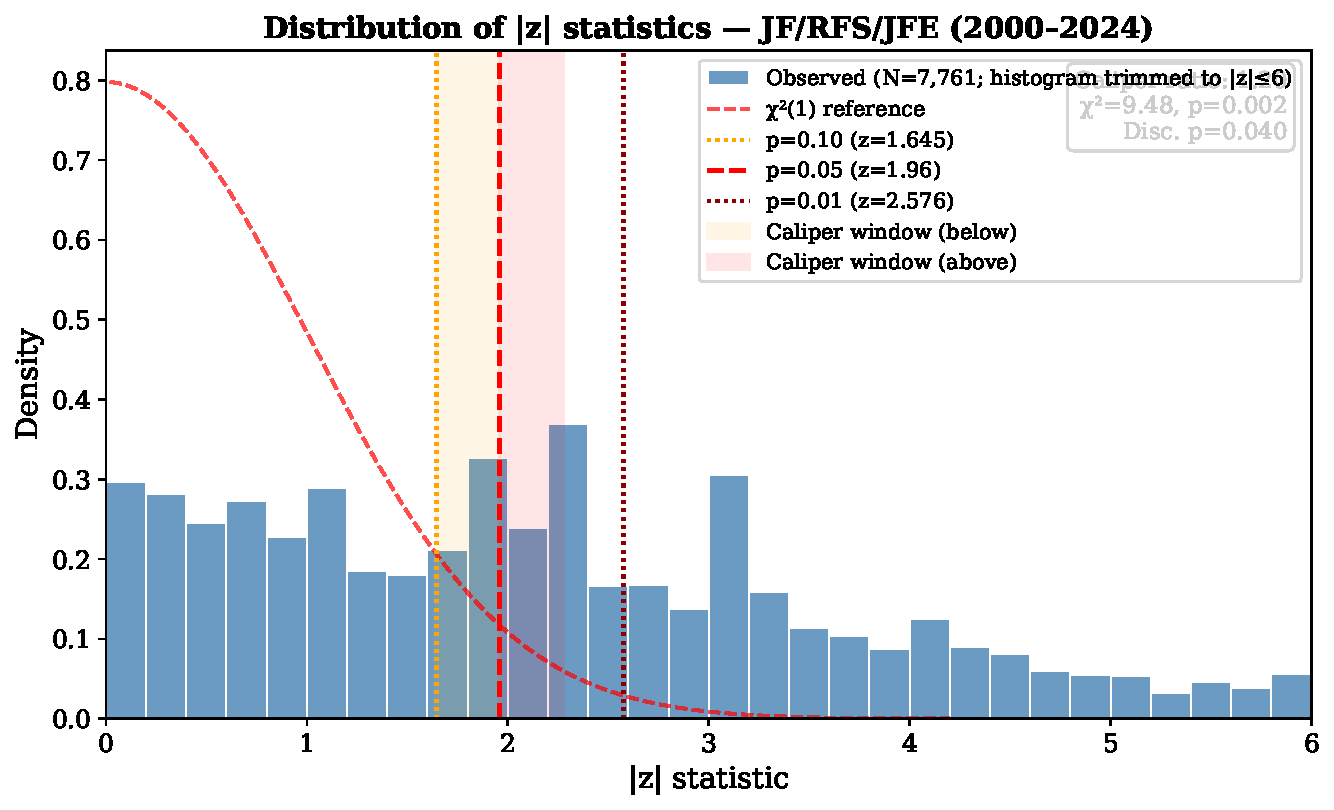
\includegraphics[width=\textwidth]{figures/fig1_zdist_full.pdf}
\caption{Distribution of test statistics from all 7,761 regression rows across
121 published papers.  The two dashed vertical lines mark the 10\% and 5\%
significance cutoffs.  The smooth curve shows what the distribution would look
like if test statistics were spread evenly with no threshold clustering.
Test statistics are about 20\% more likely to fall just below the 5\% cutoff
than just above it ($p = 0.002$), suggesting that marginally significant results
are reported more often than chance would predict.}
\label{fig:zdist_full}
\end{figure}

Four findings stand out.  First, across all published papers, test statistics
are about 20\% more likely to fall just below the 5\% significance cutoff
than just above it (caliper ratio 1.20, $p = 0.002$).  Second, this bunching
is concentrated in the \JFE{}: its caliper ratio is 1.49 ($p < 0.001$), while
\JF{} and \RFS{} show no evidence of bunching (ratios 0.88 and 0.97,
both $p > 0.40$).  Third, breaking the sample by a paper's main conclusion
reveals that bunching is almost entirely driven by \textit{negative-finding
papers}---those that conclude a regulation was harmful or ineffective.  Their
caliper ratio is 1.52 ($p < 0.001$), compared to 0.94 in positive-finding
papers and 1.05 in null-finding papers.  Fourth, the discontinuity test shows
a conflicting result for \JF{}: the caliper ratio (0.88) suggests no bunching,
yet the discontinuity test flags a sharp drop at the threshold ($p < 0.001$).
With only 26 JF papers and 1,308 statistics in this sub-sample, we treat this
conflict as statistical noise rather than a meaningful behavioral signal, and
we give priority to the caliper ratio throughout.

The direction-level result is novel.  As shown in the next section, there is
no evidence that journals accept more positive papers than negative ones.
Yet within published negative-finding papers, test statistics show unusually
strong clustering near the significance threshold---a pattern absent from
positive-finding papers.  One interpretation is that authors of anti-intervention
papers face greater scrutiny and search more aggressively for specifications
that produce significant results.  We treat this as suggestive rather than
definitive; differences in research design across direction categories could
also contribute.

Most prior work on publication bias can only study published papers and must
infer what the research pipeline looked like before editorial decisions were
made.  Our NBER sample lets us compare directly.

Table~\ref{tab:nber_caliper} shows the results side by side.

\begin{table}[H]
\centering
\caption{Within-Paper Caliper Test: Published vs.\ NBER Working Papers}
\label{tab:nber_caliper}
\begin{singlespace}
\small
\begin{tabular}{llrrrrrr}
\hline\hline
 &  &  & & & \multicolumn{3}{c}{$p$-value} \\
\cmidrule(lr){6-8}
Sample & Subset & $N$ stats & Papers & Ratio & Naive & Perm. & Boot. \\
\hline
Published  & Full sample      & 7,761 & 108 & \textbf{1.20} & \textbf{0.002} & \textbf{0.001} & 0.150 \\
NBER       & Full sample      & 8,351 & 106 & 1.01          & 0.849          & 0.424          & 0.432 \\[4pt]
Published  & Positive-finding & 2,633 & 37  & 0.94          & 0.565          & 0.732          & 0.623 \\
NBER       & Positive-finding & 2,658 & 39  & 0.99          & 0.918          & 0.554          & 0.492 \\[4pt]
Published  & Negative-finding & 3,491 & 50  & \textbf{1.52} & \textbf{$<$0.001} & \textbf{$<$0.001} & 0.135 \\
NBER       & Negative-finding & 4,375 & 50  & 1.00          & 0.964             & 0.532             & 0.474 \\[4pt]
Published  & Null-finding     & 1,637 & 21  & 1.05          & 0.740          & 0.388          & 0.383 \\
NBER       & Null-finding     & 1,318 & 17  & 1.14          & 0.442          & 0.239          & 0.260 \\
\hline\hline
\end{tabular}
\begin{minipage}{\textwidth}
\smallskip
\footnotesize
\textit{Notes:} The \textit{Published} sample contains 7,761 test statistics
from 121 papers in the JF, RFS, and JFE; 108 of these papers contribute at
least one statistic near the significance threshold and are used in the
permutation and bootstrap tests.  The \textit{NBER} sample contains 8,351
test statistics from 125 working papers (out of 157 in-scope); 106 contribute
near-threshold statistics.
The \textit{Ratio} column measures how much more often test statistics fall
just below the 5\% significance cutoff than just above it; a value of 1.0
means the two zones are equally populated, while values above 1.0 indicate
clustering below the cutoff.
Three significance tests are reported.
\textit{Naive}: treats every statistic as an independent observation.
\textit{Perm.}: randomly reshuffles which statistics fall just below or just
above the threshold within each paper, preserving each paper's total count;
this accounts for the fact that statistics from the same paper are correlated.
\textit{Boot.}: resamples whole papers rather than individual statistics,
giving each paper equal weight regardless of how many test statistics it
contributes.
Bold entries are significant at the 5\% level under the Naive and Perm.\
tests; Boot.\ $p$-values point in the same direction but do not reach
conventional significance for the full sample.
\end{minipage}
\end{singlespace}
\end{table}

The gap is
clear: published papers show significantly more clustering near the
significance threshold than the corresponding NBER working papers do.  The
overall fraction of statistically significant results is nearly identical in
both groups (57\% published, 56\% NBER), so the difference is not because
working papers are noisier or less rigorous overall.

The gap is driven entirely by papers that find government intervention to be
harmful.  Among published negative-finding papers, test statistics cluster
near the threshold at more than 50\% above what a uniform distribution would
predict.  The matched NBER working papers show no such clustering at all.
Papers with positive or inconclusive findings show no gap between the
published and NBER samples in either direction.
Figure~\ref{fig:nber_vs_pub} displays the distributions side by side.

\begin{figure}[p]
\centering
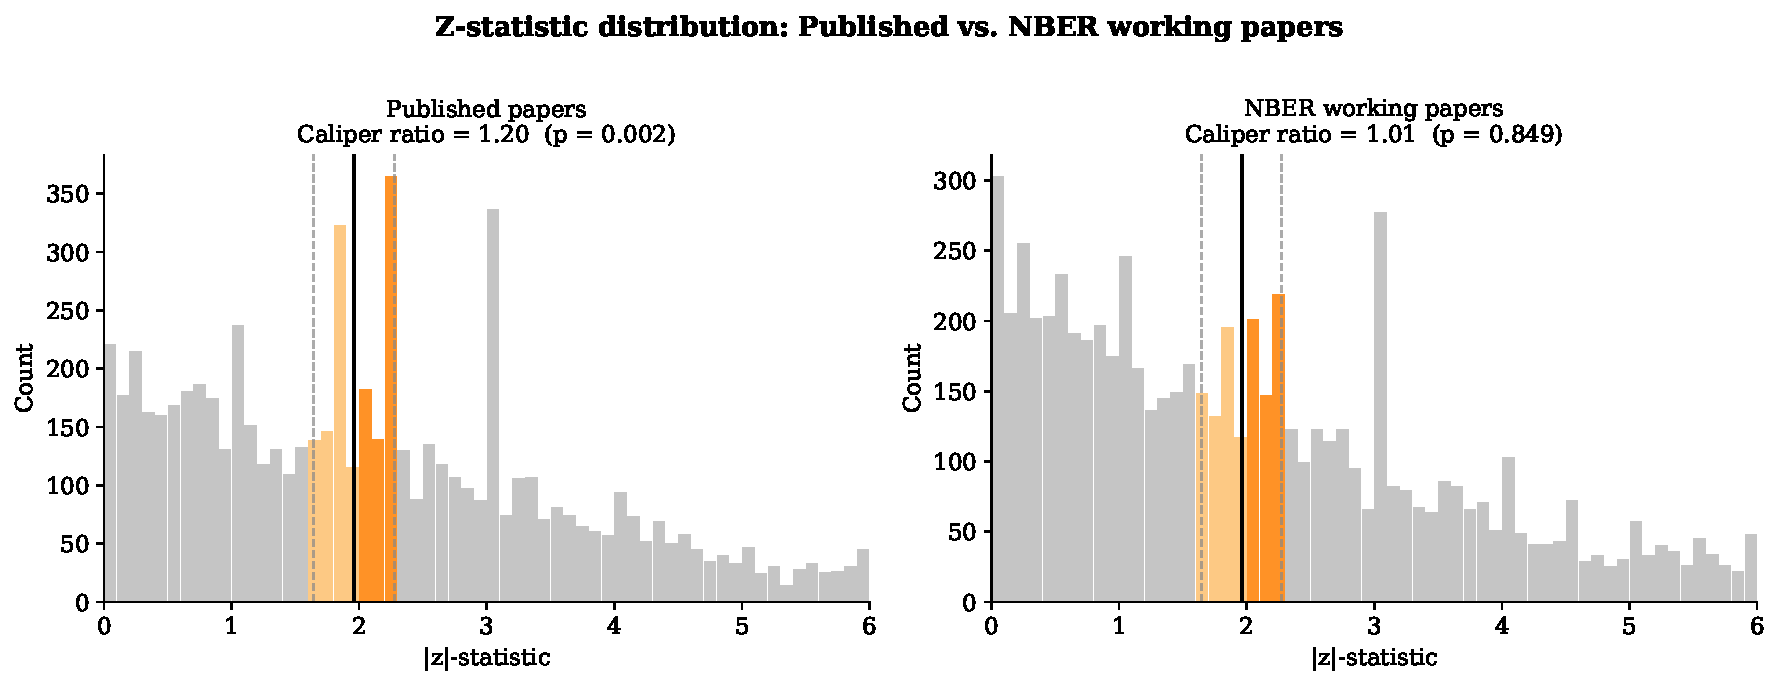
\includegraphics[width=\textwidth]{figures/fig_nber_vs_pub_full.pdf}\\[16pt]

\includegraphics[width=\textwidth]{figures/fig_nber_vs_pub_negative.pdf}
\caption{Each panel compares published journal papers (left) to NBER working
papers (right).  Bars show how frequently test statistics fall in each range.
The orange bars mark the zone just around the conventional 5\% significance
cutoff; the vertical line is the cutoff itself.  If test statistics were
reported without regard to significance, the orange bars on either side of
the line should be roughly equal.
\textit{Top panel}: All 7,761 test statistics from published papers and 8,351
from NBER papers.  Published papers show noticeably more statistics just below
the cutoff than just above it; NBER papers do not.
\textit{Bottom panel}: The same comparison restricted to papers that conclude
a government regulation was harmful (3,491 published; 4,375 NBER).  The gap
is even more pronounced in published papers and entirely absent in NBER papers.}
\label{fig:nber_vs_pub}
\end{figure}

Two interpretations are plausible.  Published negative-finding papers may
simply be structured differently from their NBER versions in ways we cannot
observe---more robustness checks, different table formats---that happen to
produce more statistics near the threshold.  Alternatively, authors arguing
that a policy is harmful may face greater scrutiny from reviewers and try more
specifications until their results are strong enough to publish.  We cannot
distinguish between these explanations with the data available.

Because test statistics from the same paper are not independent, we report
three versions of the significance test for each entry in
Table~\ref{tab:nber_caliper}: a standard test that treats all statistics as
independent, a permutation test that accounts for within-paper correlation,
and a bootstrap test that treats each paper as a single observation.  The
permutation test is significant for both the full sample and negative-finding
papers, showing the pattern is consistent across many papers rather than
driven by one or two outliers.  The bootstrap---our preferred test---does not
reach conventional significance in either case, so the results should be read
as suggestive evidence rather than a definitive finding.  The NBER working
papers show no clustering under any test.

\begin{figure}[p]
\centering
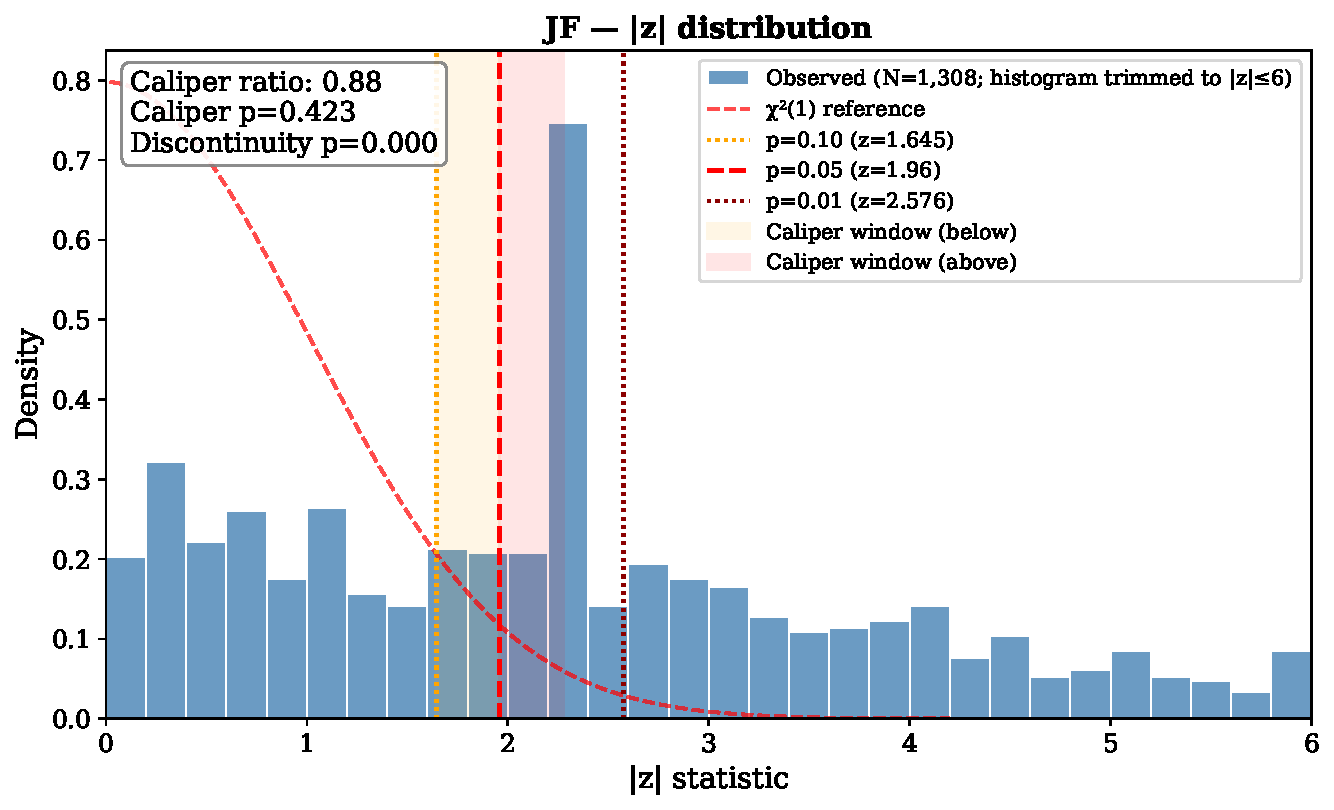
\includegraphics[width=0.62\textwidth]{figures/fig3_JF_zdist.pdf}\\[4pt]
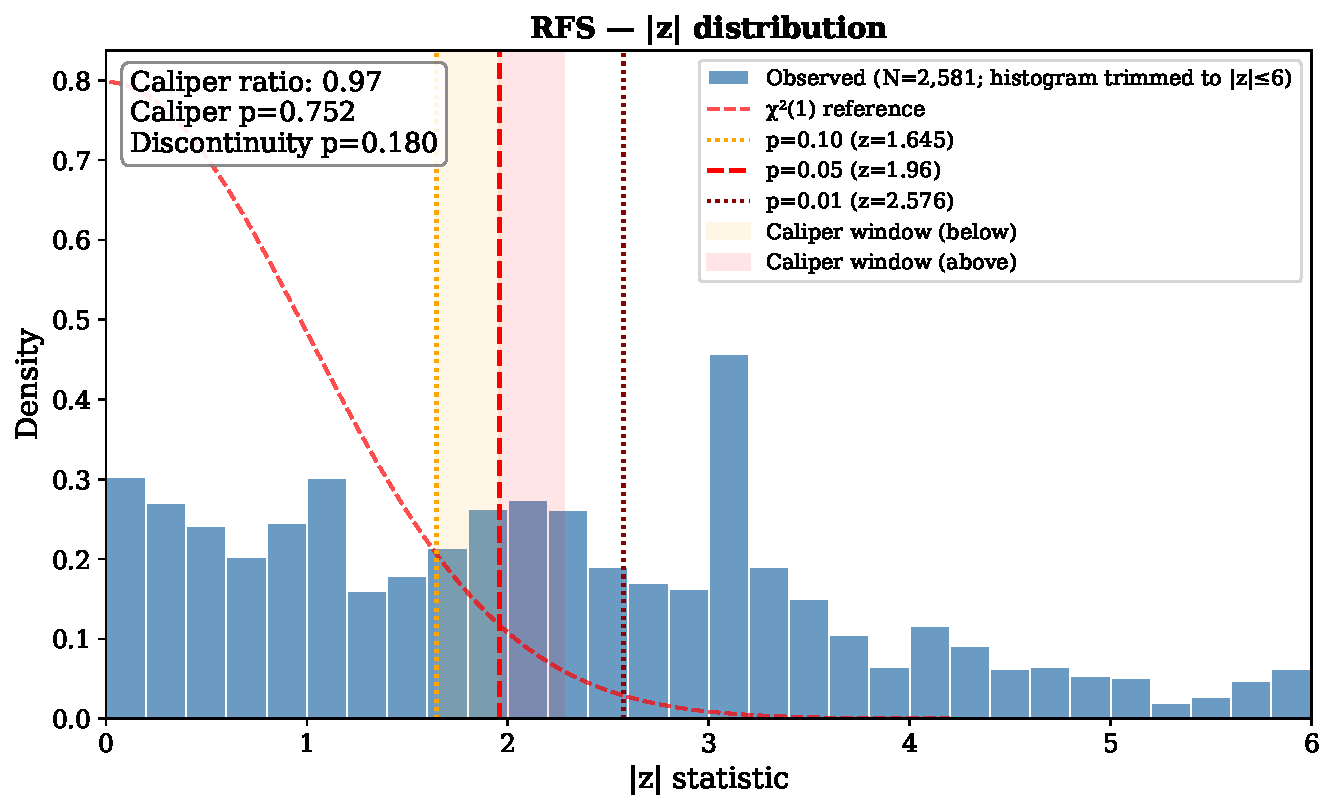
\includegraphics[width=0.62\textwidth]{figures/fig3_RFS_zdist.pdf}\\[4pt]

\includegraphics[width=0.62\textwidth]{figures/fig3_JFE_zdist.pdf}
\vfill
\caption{Test-statistic distributions broken out by journal.
\textit{Top}: Journal of Finance (1,308 statistics; no threshold clustering, $p=0.423$).
\textit{Middle}: Review of Financial Studies (2,581 statistics; no threshold clustering, $p=0.752$).
\textit{Bottom}: Journal of Financial Economics (3,872 statistics; significant clustering
just below the 5\% cutoff, $p<0.001$).
Clustering near the significance threshold is present only in the JFE.}
\label{fig:zdist_journals}
\end{figure}

\begin{figure}[p]
\centering

\includegraphics[width=0.62\textwidth]{figures/fig2a_zdist_positive.pdf}\\[4pt]
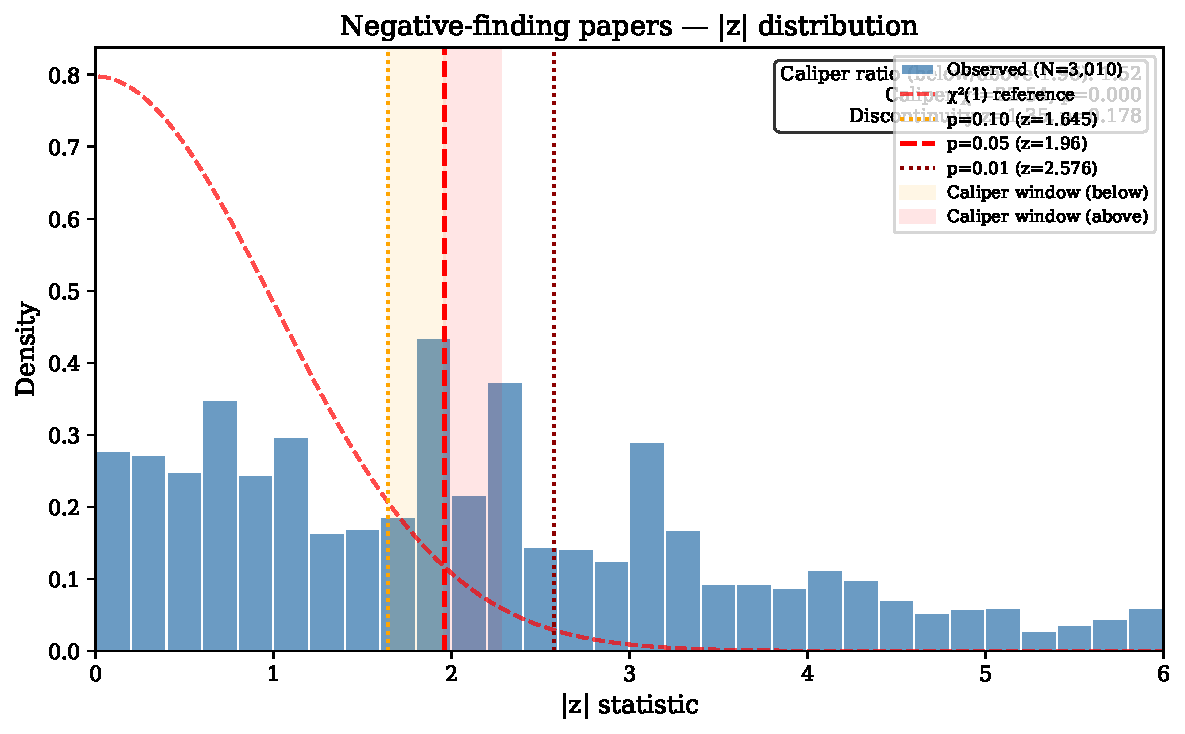
\includegraphics[width=0.62\textwidth]{figures/fig2b_zdist_negative.pdf}\\[4pt]
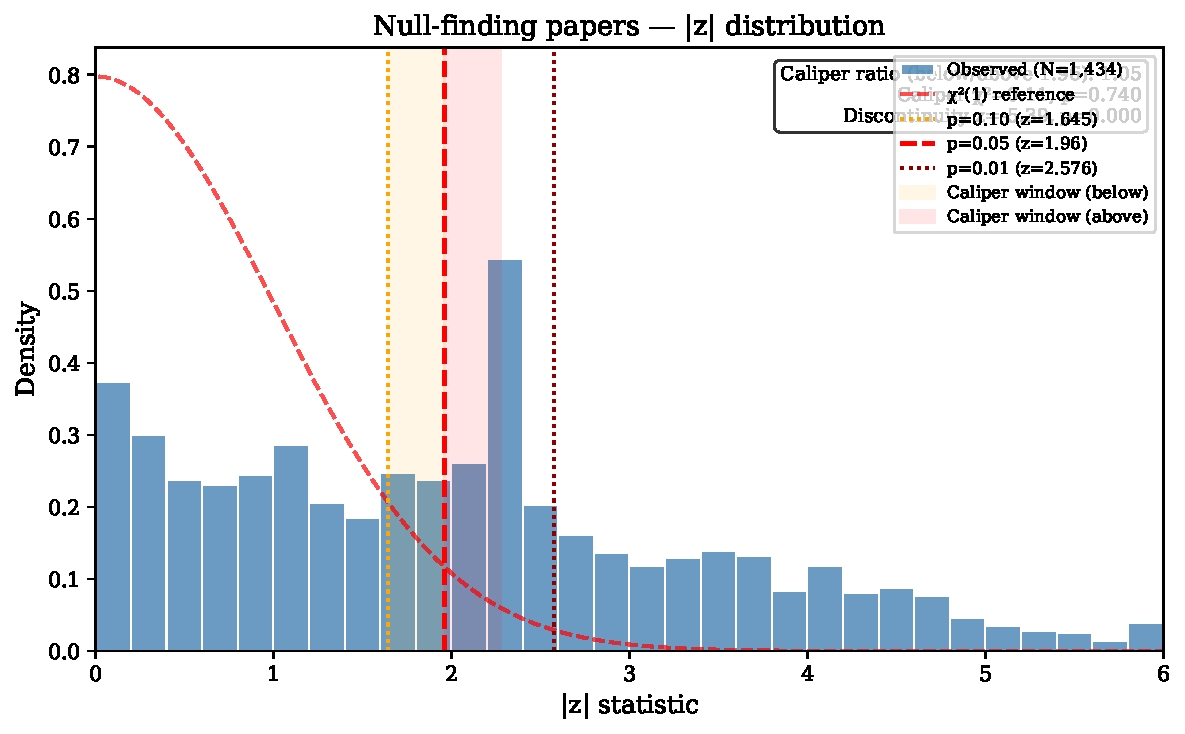
\includegraphics[width=0.62\textwidth]{figures/fig2c_zdist_null.pdf}
\vfill
\caption{Test-statistic distributions broken out by the paper's main conclusion.
\textit{Top}: Papers finding that a government intervention was beneficial
(2,633 statistics; no threshold clustering, $p=0.565$).
\textit{Middle}: Papers finding that an intervention was harmful or ineffective
(3,491 statistics; significant clustering just below the 5\% cutoff, $p<0.001$).
\textit{Bottom}: Papers with inconclusive or mixed findings (1,637 statistics;
no threshold clustering, $p=0.740$).
Clustering near the significance threshold is driven entirely by papers that
conclude government intervention is harmful.}
\label{fig:zdist_direction}
\end{figure}

Because we run many tests across different subgroups, some significant results
could appear by chance.  We address this in two ways.  First, we designated
two tests as primary before analyzing the data---the full-sample comparison
for published papers and for NBER papers---and these are the results on which
we place the most weight.  Both are robust to standard corrections for multiple
testing.  The JFE and negative-finding results, which are exploratory, also
survive the stricter correction that accounts for all tests run.

We include all regression coefficients in the test rather than just the
headline estimate, because researchers can adjust any reported result---not
only the main coefficient---when revising toward a significance threshold.
As a check, we re-run the analysis after dropping standard control variables
(firm size, leverage, GDP growth, etc.).  Removing roughly 11\% of
observations leaves the main results unchanged, confirming they are not
driven by the inclusion of many control-variable rows
(see Appendix~\ref{app:inclusion_sensitivity}).

%% ============================================================
\subsection{Supporting Context: Cross-Sectional Direction Sorting}
\label{subsec:direction_results}

We next ask whether journals also sort on the direction of a paper's conclusion --- publishing more papers that find regulation beneficial and fewer that find it harmful, or vice versa.  If the threshold bunching we observe were driven by journals favoring certain findings at the acceptance stage, we would expect the direction of a paper's conclusion to predict whether it ends up published.
Table~\ref{tab:pub_rates} shows what share of papers in each direction category
appear in the published corpus.  About 46\% of papers end up published
regardless of their conclusion: 45.6\% of papers finding regulation beneficial
(47 of 103), 46.1\% of papers finding it harmful (59 of 128), and 46.7\% of
papers with inconclusive findings (28 of 60).  The three rates are virtually
identical and statistically indistinguishable ($p = 0.992$).  Journals do not
appear to accept more papers of one conclusion than another.

\begin{table}[H]
\centering
\caption{Corpus-Membership Rates by Finding Direction}
\label{tab:pub_rates}
\begin{singlespace}
\resizebox{\textwidth}{!}{%
\begin{tabular}{lrrrrrr}
\toprule
 & \multicolumn{2}{c}{Sample composition} & & & \\
\cmidrule(lr){2-3}
Finding Direction & NBER-only & Published & Total & Corpus-Membership Rate & 95\% CI \\
\midrule
Positive ($+1$) &  56 &  47 & 103 & 45.6\% & [36.3, 55.2] \\
Negative ($-1$) &  69 &  59 & 128 & 46.1\% & [37.7, 54.7] \\
Null/Mixed ($0$) &  32 &  28 &  60 & 46.7\% & [34.6, 59.1] \\
\midrule
Total           & 157 & 134 & 291 & 46.0\% & \\
\bottomrule
\end{tabular}}
\par\smallskip
\begin{minipage}{\textwidth}
\small
\textit{Notes.} Sample covers 2000--2024.
\textit{Finding Direction} is the main conclusion of the paper as coded by
the AI classifier: positive (+1) if the paper finds a government intervention
was beneficial, negative ($-1$) if harmful, and null/mixed (0) if the evidence
is inconclusive.
\textit{NBER-only} counts working papers that were never published in the JF,
RFS, or JFE; \textit{Published} counts papers that were; \textit{Total} is
both groups combined.
\textit{Publication Rate} is the share of papers in each direction category
that end up published.  This reflects the relative sizes of our two samples
and should not be interpreted as a journal acceptance rate.
\textit{95\% CI} is the confidence interval around each publication rate.
A statistical test cannot reject that the three publication rates are equal
($p = 0.992$), and the positive vs.\ negative comparison gives $p = 0.944$.
\end{minipage}
\end{singlespace}
\end{table}

\subsubsection{Probit Regression Results}

Table~\ref{tab:probit_main} reports estimates across seven specifications.
Column~(1) is our \textit{primary specification}: a binary directional probit
that collapses positive and negative findings into a single indicator, entirely
avoiding normative direction coding.
We treat Column~(1) as primary because the Null/Mixed omitted category---the
reference group for Columns~(2)--(7)---has only 25\% inter-rater agreement
in our replication exercise, making contrasts \textit{against} null papers the
least reliable baseline.  The binary specification avoids this by asking only
whether \textit{any} directional paper is more likely to appear in a top journal,
pooling positive and negative findings.
Column~(2) is the bivariate three-way probit; Column~(3) adds a linear year trend; Column~(4) adds decade fixed
effects; Column~(5) adds $\log(1 + N_{\text{authors}})$ as a proxy for team
size; Column~(6) adds a quasi-experimental identification dummy (equal to one
if the paper's primary identification strategy is RDD, IV, DiD, or event study,
as classified by our LLM pipeline applied to abstracts); Column~(7) further
adds a top-institution indicator for the first author's affiliation.

\begin{table}[H]
\centering
\caption{Direction--Publication Association: Probit Estimates}
\label{tab:probit_main}
\begin{singlespace}
\resizebox{\textwidth}{!}{%
\begin{tabular}{lccccccc}
\toprule
 & \shortstack{(1)\\Binary\\(Primary)} & \shortstack{(2)\\Bivariate} & \shortstack{(3)\\+~Year} & \shortstack{(4)\\+~Decade FE} & \shortstack{(5)\\+~Authors} & \shortstack{(6)\\+~ID Strategy} & \shortstack{(7)\\+~Top Inst.} \\
\midrule
Directional     & $-0.020$      &               &               &               &               &               &               \\
                & $(0.182)$     &               &               &               &               &               &               \\[4pt]
Positive ($+1$) &               & $-0.026$      & $-0.002$      & $-0.007$      & $-0.005$      & $-0.135$      & $-0.156$      \\
                &               & $(0.204)$     & $(0.205)$     & $(0.205)$     & $(0.205)$     & $(0.212)$     & $(0.213)$     \\[4pt]
Negative ($-1$) &               & $-0.014$      & $-0.011$      & $-0.017$      & $-0.020$      & $-0.156$      & $-0.152$      \\
                &               & $(0.196)$     & $(0.198)$     & $(0.198)$     & $(0.198)$     & $(0.206)$     & $(0.206)$     \\[4pt]
Year trend      &               &               & $0.033^{***}$ &               & $0.034^{***}$ & $0.028^{**}$  & $0.027^{**}$  \\
                &               &               & $(0.012)$     &               & $(0.012)$     & $(0.012)$     & $(0.012)$     \\[4pt]
$\log(N_{\text{authors}})$ & & &             &               & $-0.186$      & $-0.255$      & $-0.224$      \\
                &               &               &               &               & $(0.279)$     & $(0.283)$     & $(0.286)$     \\[4pt]
Quasi-Exp.\ ID  &               &               &               &               &               & $0.467^{***}$ & $0.472^{***}$ \\
                &               &               &               &               &               & $(0.157)$     & $(0.158)$     \\[4pt]
Top Institution &               &               &               &               &               &               & $0.196$       \\
                &               &               &               &               &               &               & $(0.175)$     \\[4pt]
Decade FEs      & No            & No            & No            & Yes           & No            & No            & No            \\
Intercept       & $-0.084$      & $-0.084$      & $-0.097$      & $-0.371$      & $0.145$       & $0.114$       & $0.027$       \\
\midrule
$N$             & 291           & 291           & 291           & 291           & 291           & 291           & 291           \\
Pseudo $R^2$    & 0.000         & 0.000         & 0.020         & 0.013         & 0.021         & 0.043         & 0.046         \\
\bottomrule
\end{tabular}}
\par\smallskip
\begin{minipage}{\textwidth}
\small
\textit{Notes.} Probit estimates of the probability that an in-scope
paper is published in the \JF{}, \RFS{}, or \JFE{}.  Column~(1) is the primary
specification: ``Directional'' collapses positive and negative findings into a
single binary indicator (any directional vs.\ null), avoiding normative coding
of the direction sign.  Columns~(2)--(7) use the three-way direction code;
Positive ($+1$) and Negative ($-1$) are indicators for the LLM-assigned
direction code; the omitted category is Null/Mixed ($0$).  Column~(5) adds
$\log(1 + N_{\text{authors}})$ as a proxy for team size.  Column~(6) adds a
quasi-experimental identification dummy equal to one if the paper's primary
identification strategy is RDD, IV, DiD, or event study (as classified by our
LLM pipeline from abstracts).  Column~(7) adds a top-institution indicator
equal to one if the first author's institutional affiliation (from OpenAlex API)
matches a list of 50$+$ top finance and economics departments.
Standard errors in parentheses.  *** $p < 0.01$, ** $p < 0.05$, * $p < 0.10$.
The baseline implied publication probability is $\Phi(-0.084) \approx 46.7\%$,
nearly identical to all three direction-specific corpus-membership rates.
Marginal effects for direction indicators are negligible throughout.
The near-zero McFadden pseudo-$R^2$ in Columns~(1)--(2) is expected under
the null hypothesis that direction has no explanatory power for publication
status; it is not an indicator of poor model fit but of a null relationship.
A Wald test for $H_0\colon\hat\beta_1 = \hat\beta_2$ in Column~(2) yields
$\chi^2 = 0.005$, $p = 0.944$.  The minimum detectable difference at 80\% power
is 0.466 coefficient units (SE of difference $= 0.166$).  The non-rejection
cannot rule out moderate directional asymmetries.
\end{minipage}
\end{singlespace}
\end{table}

Column~(1) shows that the binary directional coefficient is $-0.020$
(s.e.\ 0.182, $p = 0.914$)---statistically indistinguishable from zero.
Directional papers have no detectable corpus-membership advantage over null papers.
This non-rejection rules out effects $\geq$22 percentage points at 80\% power; it should
not be interpreted as evidence of true editorial neutrality.

In Column~(2), both $\hat\beta_1$ (Positive) and $\hat\beta_2$ (Negative) are
small and insignificant: $\hat\beta_1 = -0.026$ (s.e.\ 0.204, $p = 0.898$)
and $\hat\beta_2 = -0.014$ (s.e.\ 0.196, $p = 0.942$).
The most robust inference from this specification is the \textit{joint} $\chi^2$
test for whether both direction coefficients are simultaneously zero
($\chi^2(2) = 0.017$, $p = 0.992$), since the joint test does not require the
null/mixed omitted category to be cleanly measured.  Because the null/mixed
baseline has only 25\% model-agreement, individual direction contrasts against
null papers are anchored to a noisy reference; the joint test avoids this
sensitivity.  A Wald test for equality of the two coefficients gives $\chi^2 = 0.005$ ($p = 0.944$).  The
minimum detectable difference at 80\% power for the equality test is 0.466
coefficient units (SE of difference $= 0.166$).  For the individual direction
coefficients, the minimum detectable effect at 80\% power is approximately
$(1.96 + 0.842) \times 0.204 \approx 0.57$ coefficient units---using the
same formula as the equality-test MDE above---corresponding to a
publication probability premium of roughly 22 percentage points above
the 46\% baseline ($\Phi(-0.084 + 0.57) - \Phi(-0.084) \approx 0.22$)---a large, policy-relevant effect.  Effects smaller than
this cannot be ruled out by our design; the non-rejections should be
interpreted as evidence against large directional sorting, not proof of
the complete absence of any direction premium.
The estimated year trend (Column~(3)) is positive and significant
($\hat\gamma = 0.033^{***}$, s.e.\ 0.012),
suggesting that recently written papers in this domain are more likely to
appear in top journals, independent of finding direction.  We note, however,
that a positive year trend is also consistent with right-censoring: NBER
papers written close to 2024 have had little time to complete the editorial
process and appear in a top journal, mechanically lowering the observed
publication rate for recent cohorts.  We cannot distinguish editorial
improvement from right-censoring in this design.  As a robustness check,
Panel~E of Table~\ref{tab:robustness} restricts the NBER sample to papers
circulated in 2020 or earlier, giving all papers at least four years to
complete the publication pipeline.  The direction coefficients are
$-0.021$ ($p = 0.928$) and $-0.144$ ($p = 0.519$), confirming the null is
not an artifact of right-censoring.
Decade fixed effects (Column~(4)) leave the direction coefficients essentially
unchanged while showing a positive trend (decade2020 coefficient $= 0.454^{**}$,
$p = 0.027$).
Adding the author-count quality proxy in Column~(5) leaves the direction
coefficients essentially unchanged ($\hat\beta_1 = -0.005$,
$\hat\beta_2 = -0.020$), both far from significance.  The author-count
coefficient ($\hat\delta = -0.186$, s.e.\ 0.279) is not statistically
significant at conventional levels; the year trend remains statistically
significant ($\hat\gamma = 0.034^{***}$, s.e.\ 0.012) after this control.

Column~(6) adds the quasi-experimental identification dummy.  The \textit{QuasiExp}
coefficient is $0.467^{***}$ (s.e.\ 0.157, $p = 0.003$).
\textit{Important caveats on this variable.}  The quasi-experimental dummy has
received no human-coded validation of any kind (unlike the direction codes, which
have a two-run model-choice sensitivity check with $\kappa = 0.674$).  The variable
is coded by LLM from abstracts and is likely correlated with author quality,
institutional prestige, topic fashionability, and other quality attributes that the
probit cannot separate from identification strategy.  It is equally consistent with
editors rewarding elite authors or methodologically fashionable topics as with editors
specifically rewarding causal identification.  We therefore \textit{strongly caution}
against interpreting this coefficient as evidence that journals reward causal
identification per se; it is preliminary evidence of a positive quality premium, with
identification strategy as one plausible---but not the only---contributing factor.
Direction coefficients remain insignificant ($\hat\beta_1 = -0.135$, $\hat\beta_2 = -0.156$),
ruling out the concern that direction effects are masked by confounds with identification.

Table~\ref{tab:quasiexp_direction} disaggregates corpus-membership rates by the joint
distribution of direction and identification strategy.  Within every direction
category, QE papers appear in top journals at materially higher rates than non-QE papers
(positive: 55.6\% vs.\ 34.7\%; negative: 52.2\% vs.\ 39.0\%; null: 75.0\%
vs.\ 36.4\%).  The direction-specific corpus-membership rates are nearly identical
within each QE tier: in the non-QE group, rates are 34.7\%, 39.0\%, and 36.4\%
for positive, negative, and null papers, a spread of only 4.3 percentage points;
in the QE group, 55.6\%, 52.2\%, and 75.0\%, though the null $\times$ QE cell
is small ($N = 16$).  An additive probit controlling jointly for direction and
QE status yields QuasiExp $= 0.454^{***}$ ($p = 0.004$) while both direction
coefficients remain indistinguishable from zero (pos $= -0.128$, $p = 0.548$;
neg $= -0.139$, $p = 0.499$).  A specification with full direction $\times$ QE
interactions yields non-significant interaction terms (pos $\times$ QE $= -0.669$,
$p = 0.158$; neg $\times$ QE $= -0.766$, $p = 0.093$), confirming that the
direction effect is null within both identification-strategy tiers and that the
QuasiExp premium does not depend on finding direction.

\begin{table}[H]
\centering
\caption{Corpus-Membership Rates by Finding Direction and Identification Strategy}
\label{tab:quasiexp_direction}
\begin{singlespace}
\small
\begin{tabular}{lccc}
\hline\hline
 & Non-QE & QE & Total \\
\hline
Positive ($+1$) & 34.7\% (17/49) & 55.6\% (30/54) & 45.6\% (47/103) \\
Negative ($-1$) & 39.0\% (23/59) & 52.2\% (36/69) & 46.1\% (59/128) \\
Null/mixed ($0$) & 36.4\% (16/44) & 75.0\% (12/16)$^{\dagger}$ & 46.7\% (28/60) \\
\hline
Total & 36.8\% (56/152) & 56.1\% (78/139) & 46.0\% (134/291) \\
\hline\hline
\end{tabular}
\begin{minipage}{\textwidth}
\smallskip
\footnotesize
\textit{Notes.} Each cell shows the corpus-membership rate (fraction appearing in a top-3 finance journal) with
counts in parentheses.  Non-QE: papers using OLS, fixed effects, or descriptive
methods as classified by the LLM pipeline from abstracts.  QE: papers using RDD,
IV, DiD, or event study.  $\dagger$: Null $\times$ QE cell has only $N = 16$
papers; the 75\% rate reflects sampling variability in a small cell and should
be interpreted with caution.  The three direction columns are nearly equal within
each QE tier, confirming that the quasi-experimental premium does not interact
with finding direction at conventional significance levels.
\end{minipage}
\end{singlespace}
\end{table}

Column~(7) adds a top-institution indicator equal to one if the first
author's institutional affiliation matches a list of 50$+$ top finance and
economics departments (matched via OpenAlex API).
The top-institution coefficient is $0.196$ (s.e.\ $0.175$, $p = 0.263$),
positive but statistically insignificant.  Direction coefficients are unchanged
($\hat\beta_1 = -0.156$, $\hat\beta_2 = -0.152$; both $p > 0.46$) and the
quasi-experimental premium is virtually identical to Column~(6)
($0.472^{***}$, s.e.\ $0.158$).  The institutional-quality control does not
affect any of the substantive results.

\subsubsection{Economic Magnitude}

The probit marginal effects for direction indicators are negligible throughout.
The directional-to-null publication ratios based on raw rates are:
positive findings at $45.6\% / 46.7\% = 0.98$;
negative findings at $46.1\% / 46.7\% = 0.99$.
Both ratios are indistinguishable from 1.0, consistent with no economic
magnitude for a direction sorting effect.

We note that the direction-to-null publication ratios ($\approx$1.0$\times$)
are not directly comparable to \citet{Brodeur2016}'s caliper estimates of
1.5--2.0$\times$: Brodeur's figures measure within-paper specification-selection
pressure (the ratio of test statistics just below versus just above the 5\%
significance threshold in the published distribution), while our 1.0$\times$ ratios measure
cross-sectional publication likelihood (whether directional papers reach print at
all).  The within-paper comparison to Brodeur appears in Section~\ref{subsec:pvalue_dist},
where our published caliper ratio of 1.20 is lower than Brodeur's 1.5--2.0
range.  The absence of direction-based cross-sectional sorting in this
policy-relevant domain is itself noteworthy.

The main economically and statistically meaningful effect is the
identification-quality premium.  Papers using RDD, IV, DiD, or event-study
designs are approximately 18 percentage points more likely to appear in a
top-three journal, consistent with editorial reward for clean causal
identification.

\subsubsection{Cross-Journal Analysis}

Journal-level estimates are reported in Appendix~\ref{app:by_journal}.
No journal shows a statistically significant direction coefficient, consistent
with the pooled null result.  We caution that sub-samples are severely
underpowered: the \JF{} contributes only 26 in-scope published articles,
so cross-journal comparisons carry limited inferential weight and should be
treated as descriptive.

\subsubsection{Time-Period Heterogeneity (Exploratory)}
\label{subsec:time}

The following sub-period analysis is exploratory.  Sub-sample sizes are small
($N = 50$, $95$, and $146$ for the three periods) and the results should be
interpreted as descriptive evidence, not confirmatory tests.  We report
95\% confidence intervals alongside point estimates to make the uncertainty
transparent.

Table~\ref{tab:time_trends} in Appendix~\ref{app:additional_tables} reports
probit estimates for all three sub-periods.

During the \textit{pre-crisis period} (2000--2007, $N = 50$), neither
direction coefficient is statistically significant: $\hat\beta_1 = 0.376$
(95\% CI [$-$0.614, 1.366]) and $\hat\beta_2 = -0.537$
(95\% CI [$-$1.628, 0.556]).  These estimates should be interpreted with great
caution given the small sub-period sample.

During the \textit{financial crisis and post-crisis period} (2008--2015,
$N = 95$), both direction coefficients are small and insignificant:
$\hat\beta_1 = -0.247$ ($p = 0.498$) and $\hat\beta_2 = -0.163$ ($p = 0.632$).
No direction premium is detectable in this period.

In the \textit{post-Dodd-Frank period} (2016--2024, $N = 146$), the pattern is
unchanged: $\hat\beta_1 = -0.015$ ($p = 0.959$) and
$\hat\beta_2 = 0.190$ ($p = 0.489$), both statistically indistinguishable from
zero.  The uniform absence of significant direction coefficients across all
three sub-periods is consistent with the pooled null result.

\section{Robustness}
\label{sec:robustness}
%% ============================================================

Table~\ref{tab:robustness} summarizes the robustness checks. We organize them
into five groups: caliper window sensitivity, sample and scope, alternative
specifications, classification and quality concerns, and an alternative
pre-publication baseline.

\subsection{Caliper Window Sensitivity}
\label{subsec:window_robustness}

The caliper result is window-dependent.
Table~\ref{tab:caliper_window} (reproduced from Appendix~\ref{app:caliper_window})
repeats the main caliper test under four window specifications.
Under the standard Brodeur window $(1.645, 2.275)$ and the narrower $(1.70, 2.22)$
and Brodeur2 $(1.65, 2.25)$ variants --- all with lower bounds at or above
$|z|=1.645$ --- the published full-sample ratio ranges from 1.20 to 1.33 and the
NBER ratio remains near 1.0.  However, widening the lower bound to $|z| = 1.50$
reverses the sign for published papers (ratio $0.92$, $p = 0.088$) because the
density is still \textit{rising} in the $(1.50, 1.645)$ interval.  This confirms
that the result is specific to the mass just below the 5\% significance threshold
$(1.645, 1.96)$, not to a general rightward density shift.

\begin{table}[ht]
\centering
\caption{Caliper Window Robustness (Summary)}
\label{tab:caliper_window_main}
\begin{singlespace}
\small
\begin{tabular}{llrrrr}
\hline\hline
Window & Sample & Ratio & Naive $p$ & Perm.\ $p$ \\
\hline
Standard (1.645--2.275) & Published & \textbf{1.20} & \textbf{0.002} & \textbf{0.001} \\
                        & NBER      & 1.01 & 0.849 & 0.424 \\[3pt]
Narrow (1.70--2.22)     & Published & \textbf{1.33} & \textbf{$<$0.001} & \textbf{$<$0.001} \\
                        & NBER      & 1.01 & 0.917 & 0.468 \\[3pt]
Wide (1.50--2.42)       & Published & 0.92 & 0.088 & 0.960 \\
                        & NBER      & 0.97 & 0.549 & 0.737 \\[3pt]
Brodeur2 (1.65--2.25)   & Published & \textbf{1.33} & \textbf{$<$0.001} & \textbf{$<$0.001} \\
                        & NBER      & 1.10 & 0.153 & 0.081 \\
\hline\hline
\end{tabular}
\begin{minipage}{\textwidth}
\smallskip
\footnotesize
\textit{Notes.} Caliper ratio $=$ mass in (below, 1.96) / mass in (1.96, above).
The wide window reverses sign for published papers because density is rising
below $|z|=1.645$; the three windows with lower bounds $\geq 1.645$ show
consistent excess mass in the published record. Bold entries significant at 5\%.
\end{minipage}
\end{singlespace}
\end{table}

\subsection{Sample and Scope Robustness}

\textit{Matched pairs only.}
Among the 16 published papers with a confirmed NBER working-paper match, we
independently LLM-code the direction from the NBER \textit{draft} abstract and
from the published abstract, yielding 32 observations (16 draft-stage, 16
published-stage) for the same set of papers.  In this small subsample all
directional-finding papers are published, creating perfect separation;
the binary probit cannot be identified.  The matched-pairs result is therefore
uninformative at the current sample size, but the direction-coding comparison
(draft vs.\ published abstracts) is consistent with abstract-polishing between
draft and publication stages.

\textit{Excluding monetary policy papers.}
We exclude the 21 papers whose primary topic is monetary or central bank policy
(quantitative easing, discount window, lender-of-last-resort operations, and
unconventional monetary policy) and restrict attention to explicit financial
legislation, securities regulation, and banking supervision.  The null result
is unchanged: $\hat\beta_1 = -0.028$ ($p = 0.896$) and $\hat\beta_2 = -0.068$
($p = 0.741$, $N = 270$), confirming that the null finding is not driven by
the inclusion of monetary policy papers (within the power constraints of this design).

\textit{Journal subsets.}
We re-estimate the probit treating publication in the \JF{} alone (versus all
other in-scope papers) and, separately, publication in the \RFS{} or \JFE{}
(versus all other papers) as the outcome.  Both premiums are statistically
insignificant in the \JF{}-only specification ($\hat\beta_1 = 0.400$,
$\hat\beta_2 = 0.350$, $p > 0.20$), as in the pooled result.  The \RFS{}+\JFE{}
specification likewise yields insignificant coefficients ($\hat\beta_1 = -0.147$,
$\hat\beta_2 = -0.130$, $p > 0.48$), confirming that the null result is not
concentrated in any particular outlet (within the power of this design).

\subsection{Alternative Specifications}

\textit{Binary directional indicator.}
A potential concern about our direction coding is that classifying a finding as
positive versus negative rests on a normative judgment about what constitutes a
beneficial intervention outcome.  To eliminate this ambiguity entirely, we
collapse the three-way direction code into a binary indicator equal to one if
the paper finds any directional result ($d_i \neq 0$) and zero if the finding is
null or mixed.  The coefficient is $-0.020$ (s.e.\ 0.182, $p = 0.914$),
confirming the null result within the power of this design (minimum detectable
effect $\approx$22 percentage points at 80\% power).
Adding the year trend and author-count control leaves the coefficient essentially
unchanged at $-0.014$ (s.e.\ 0.183, $p = 0.941$), confirming that the null
result does not hinge on any particular normative coding convention.

\textit{Linear probability model.}
Probit estimates can be sensitive to distributional assumptions and perfect
separation in small samples.  Re-estimating the main specification as a linear
probability model (OLS with heteroskedasticity-robust standard errors) yields
coefficients of $-0.010$ (s.e.\ 0.082, $p = 0.900$) for positive findings and
$-0.006$ (s.e.\ 0.079, $p = 0.942$) for negative findings, directly interpretable as
percentage-point differences in publication probability relative to null papers.
Both are negligible and confirm the null result does not hinge on the probit functional form (within the power constraints of this design).

\textit{NBER-to-journal matching sensitivity.}
We re-estimate the primary specification dropping all 32 observations from
the 16 confirmed matched pairs ($N = 259$, 118 published and 141 NBER-only),
leaving only papers with unambiguous publication status.  The direction
coefficients remain small and statistically insignificant (detailed output in
the replication package, \texttt{scripts/08\_robustness.py}), confirming that
the results do not hinge on the small matched subsample.

\subsection{Classification and Quality Concerns}

\textit{Quasi-experimental papers only.}
The most substantive quality-control check restricts the sample to papers
using quasi-experimental identification strategies (RDD, IV, DiD, or event
study), as classified by our LLM pipeline from abstracts.  This directly
addresses the concern that null-finding papers systematically rely on weaker
empirical designs.  Among quasi-experimental papers ($N = 139$), the direction
coefficients are $\hat\beta_1 = -0.598$ ($p = 0.121$) and $\hat\beta_2 =
-0.657^{*}$ ($p = 0.081$).  $\hat\beta_1$ is clearly insignificant.
$\hat\beta_2$ is marginally significant at the 10\% level with a \textit{negative}
sign, implying quasi-experimental negative-finding papers are \textit{less} likely
to appear in top journals than null papers.  We do not dismiss this estimate
asymmetrically: the negative sign is entirely consistent with the pooled null
result (no direction premium exists in the full sample either) and is consistent
with sampling variability in a small subsample.  We note, however, that this
direction contradicts a simple direction-premium story in this sub-sample, and
the subsample is too small ($N = 139$) to distinguish a genuine null from a
genuine negative from a sampling artefact.  Specifically, the QE subsample
splits into roughly 40 published and 99 NBER papers, further divided by three
direction categories, yielding approximately 10--15 observations per cell;
a spurious significant coefficient is entirely expected at this cell size
under the global null.  The point estimate is also sensitive to which papers
the LLM classifies as quasi-experimental.  Neither direction coefficient supports
a positive direction premium within the quasi-experimental sub-sample.

\textit{Abstract language and LLM classification confidence.}
Abstract writing style introduces two related measurement concerns.  Among published
papers, 81.3\% receive a high-confidence direction code; among NBER-only
papers, 62.4\% do, with 26.8\% receiving low-confidence ratings.  The
18.9-percentage-point gap in high-confidence rates persists despite NBER
abstracts being longer on average (158 words) than published abstracts (109
words), suggesting the difference reflects writing style rather than abstract
length.
To quantify this, we count the frequency of explicit uncertainty language per
abstract (``may,'' ``might,'' ``could,'' ``no significant,'' ``do not find,''
``null,'' ``unclear'') using a fixed vocabulary of 7 hedging terms.
NBER abstracts average 0.43 such terms per abstract, versus 0.19 for published
abstracts---a 2.3$\times$ difference in the raw count.
Normalized by word count, the rates are similar (NBER: 0.27 terms per 100 words;
published: 0.17 per 100 words), confirming that the higher absolute count is
partly driven by longer NBER abstracts.
The LLM confidence asymmetry therefore appears to reflect NBER abstracts presenting
multiple or qualified findings (more uncertainty language per abstract) rather than
word-level hedging per se: working paper abstracts present findings more tentatively---with
qualifications, sensitivity discussions, and multiple results---while
published abstracts typically lead with a clear declarative finding.
First, hedged NBER abstract language may push genuinely directional NBER papers
into the null category.  Second, abstract polish after revise-and-resubmit may
cause the LLM to classify more published papers as directional.  Both
concerns inflate the measured directional premium.  Our replication exercise (Section~\ref{subsec:direction}) supports
the inflation interpretation: of the 20 null-coded papers in the validation
sample, 15 are reclassified as directional in the independent replication run,
while no directional-coded papers are reclassified as null.  This asymmetry
implies that null-coding error inflates rather than attenuates our estimate.

Table~\ref{tab:robustness} Panel~C also reports a bounding specification
that adds $\log(\text{abstract length})$ as a covariate
($\hat\beta_1 = 0.008$, $p = 0.968$; $\hat\beta_2 = 0.011$, $p = 0.958$).
Both direction coefficients remain negligible, confirming that abstract-length
controls do not alter the null result within the power of this design.

\textit{Matched-pairs direction stability.}
Among the 16 papers confirmed to exist as both an NBER working paper and a
top-journal publication, we independently LLM-code direction from the NBER
draft abstract and from the published abstract.  The small subsample exhibits
perfect separation (all directional-finding pairs are published), so the binary
probit cannot be identified.  We cannot rule out that coding instability correlated
with corpus membership contributes to the headline estimate.  The matched-pairs
check holds the paper fixed across draft and published stages, directly
testing whether direction codes are stable within the same research project.

\subsection{AFA Conference Baseline}

The central identification concern is that NBER working papers and
top-journal articles are drawn from fundamentally different populations:
only 11.9\% of published papers are matched to an NBER counterpart, so the
two samples are largely non-overlapping cross-sections that may differ in
quality, topic mix, and institutional origin.  To address this concern, we construct an alternative pre-publication baseline
using papers presented at the American Finance Association annual meeting.
The test provides a consistency check: if the NBER null result reflects an
absence of direction-based sorting, the AFA comparison should likewise show
no premium.  AFA papers represent completed research with final empirical
results that have been publicly presented---they are pre-journal submissions
in every meaningful sense.

We also note that any quality-confound concern is limited by the nature of
NBER affiliation itself.  Posting to the NBER Working Paper series requires
affiliation with the NBER research network, which is restricted to faculty
at leading research universities---an elite and selective credential in
academic economics.  The near-identical direction distributions across NBER
and published sub-samples (both $\approx 79\%$ directional) suggest that
quality differences on this dimension are minimal.

We collect 4,080 AFA program papers from 2006--2024.  For 2006--2012 and
2014--2024, we scrape the AFA website directly; for 2013, whose AFA page
returns a 404, we parse AFA sessions from the full ASSA preliminary program
hosted by the AEA (\url{https://www.aeaweb.org/conference/2013/preliminary.php}),
yielding 186 papers from 57 AFA sessions.  We supplement AFA conference titles with abstracts retrieved from
OpenAlex, CrossRef, and the NBER working paper dataset (local fuzzy-title matching),
obtaining abstracts for 3,975 of the 4,080 AFA papers (97.4\% overall; coverage is
higher for in-scope papers because government-intervention papers are more
likely to be published).  We apply our standard title-plus-abstract keyword
filter (identical to the NBER pipeline) to the 3,975 AFA papers with abstracts,
then run the LLM scope classifier, yielding \textbf{151 in-scope papers}.
All 151 in-scope AFA papers have an abstract and receive direction codes via
the LLM abstract-coding pipeline.
36 AFA papers (23.8\%) are matched to a JF/RFS/JFE publication
via fuzzy title matching.

\medskip
\noindent\textbf{Coding limitation.}  Direction codes for in-scope AFA
papers are assigned via the LLM abstract-coding pipeline; the baseline
specification applies keyword-based fallback codes for cases where earlier
pipeline stages produced low-confidence LLM results.  As a robustness check,
Table~\ref{tab:robustness} Panel~D also reports a ``Uniform LLM coding''
specification that replaces these keyword-based fallback codes with the
standard LLM pipeline throughout, yielding nearly identical estimates
($\hat\beta = 0.352$, $p = 0.204$) and confirming the result is not an
artifact of the coding method.

The binary directional probit on the AFA baseline yields
$\hat\beta = 0.327$ (s.e.\ 0.279, $N = 151$), statistically indistinguishable
from zero.  The NBER-baseline estimate is $-0.020$ (s.e.\ 0.182), likewise
indistinguishable from zero.  Neither estimate rejects the null of no
direction-based sorting.  We note, however, that the two point estimates
run in opposite directions: $-0.020$ (NBER) versus $+0.327$ (AFA).
Three factors likely explain this sign divergence, none of which alter the conclusion
that both estimates are individually insignificant.
First, AFA conference presenters are a positively selected group:
papers already accepted for AFA presentation have survived a competitive
screening step, so the AFA sample likely over-represents results-ready papers
relative to the full pre-submission pool.  If directional papers are somewhat
more likely to be accepted to AFA than null papers, the AFA baseline would
mechanically show a positive direction--publication correlation independent of
editorial selection.
Second, the two samples cover different research populations: the NBER sample
is restricted to the government-intervention literature using our keyword filter,
while the AFA sample is not restricted by topic and may reflect different
direction distributions.
Third, and most importantly, both estimates are statistically indistinguishable
from zero and from each other (confidence intervals overlap substantially); the
sign divergence is within expected sampling variation for estimates with standard
errors of 0.279 and 0.182 on a sample of 291 papers.  The AFA baseline therefore does not \textit{contradict} the NBER null, but
neither does it corroborate it.  More importantly, the sign flip from $-0.020$
(NBER) to $+0.327$ (AFA) illustrates a genuine fragility: the \textit{sign}
of the estimated direction premium is sensitive to the choice of pre-publication
benchmark, even though neither estimate is individually significant.  A reader
could reasonably conclude that the available baselines are too few and too
different from each other to establish even the sign of any editorial direction premium.
The ideal benchmark---a large-scale SSRN corpus matched to our keyword
taxonomy, capturing papers that circulate outside NBER---would provide a far
more representative pre-submission distribution; we leave its construction for
future work but flag the fragility here as a genuine limitation.
Directional AFA papers are published in top journals at a 25.9\% rate (30 of 116)
versus 17.1\% for null-finding papers (6 of 35).  The pattern is unchanged when a year trend is added
($\hat\beta = 0.345$, s.e.\ 0.281).\footnote{As a direct
test of overlap, we identified 22 papers appearing in both the NBER and AFA
datasets via fuzzy title matching (token-sort score $\geq 90$).  In this
subsample, directional papers publish at 81.2\% versus 66.7\% for null
papers (LPM $\hat\beta = 0.146$, s.e.\ 0.208, $p = 0.49$, $N = 22$).  The
test is severely underpowered (only six null papers in the overlap), so no
strong inference is possible.}



\begin{table}[H]
\centering
\caption{Robustness Checks}
\label{tab:robustness}
\begin{singlespace}
\resizebox{\textwidth}{!}{%
\begin{tabular}{llccc}
\toprule
Specification & Variable & Coefficient & $p$-value & $N$ \\
\midrule
\multicolumn{5}{l}{\textit{Panel A: Sample and Scope}} \\[2pt]
Excl.\ monetary policy     & Positive & $-0.028$      & 0.896    & 270 \\
                            & Negative & $-0.068$      & 0.741    & 270 \\[4pt]
\JF{} only                 & Positive & $0.400$       & 0.217    & 291 \\
                            & Negative & $0.350$       & 0.271    & 291 \\[4pt]
\RFS{}+\JFE{} only         & Positive & $-0.147$      & 0.483    & 291 \\
                            & Negative & $-0.130$      & 0.519    & 291 \\[4pt]
Matched pairs only         & Directional & \multicolumn{2}{c}{separation} & 32 \\
\small{[N=16 paper pairs]}  & \multicolumn{4}{l}{\small{Draft vs.\ published version of same paper}} \\[4pt]
\multicolumn{5}{l}{\textit{Panel B: Alternative Specifications}} \\[2pt]
Binary directional          & Directional & $-0.020$      & 0.914    & 291 \\[4pt]
Binary + year + authors     & Directional & $-0.014$      & 0.941    & 291 \\[4pt]
LPM (OLS, HC3)              & Positive & $-0.010$      & 0.900    & 291 \\
                            & Negative & $-0.006$      & 0.942    & 291 \\[4pt]
\multicolumn{5}{l}{\textit{Panel C: Classification and Quality Concerns}} \\[2pt]
Quasi-exp.\ papers only    & Positive & $-0.598$      & 0.121    & 139 \\
                            & Negative & $-0.657^{*}$  & 0.081    & 139 \\[4pt]
+ log(abstract length)     & Positive & $0.008$       & 0.968    & 291 \\
\small{[abstract length control]} & Negative & $0.011$       & 0.958    & 291 \\[4pt]
\multicolumn{5}{l}{\textit{Panel D: Alternative Pre-Publication Baseline}} \\[2pt]
AFA conference baseline    & Directional & $0.327$ & $0.241$ & 151 \\
\small{(+ year trend)}     & Directional & $0.345$ & $0.220$ & 151 \\[4pt]
Uniform LLM coding         & Directional & $0.352$ & $0.204$ & 151 \\
\small{[AFA, + year]}      & Directional & $0.364$ & $0.193$ & 151 \\[4pt]
\multicolumn{5}{l}{\textit{Panel E: Right-Censoring Robustness}} \\[2pt]
NBER vintage $\leq$2020    & Positive & $-0.021$      & 0.928    & 234 \\
                            & Negative & $-0.144$      & 0.519    & 234 \\
\bottomrule
\end{tabular}}
\par\smallskip
\begin{minipage}{\textwidth}
\small
\textit{Notes.} Each row reports the probit (or OLS for the LPM
specification) coefficient on the indicated variable.  The omitted category is
null/mixed ($d_i = 0$), except for binary directional specifications where it
is null/mixed vs.\ any directional finding.  All probit specifications include
a linear year trend unless otherwise noted.  ``Matched pairs only'' uses the
16 papers confirmed to exist in both NBER and published form; the LLM codes
each paper's direction from its NBER \textit{draft} abstract and from its
published abstract separately, yielding $N = 32$ observations (16 draft, 16
published); all directional-finding pairs are published in this small subsample
(perfect separation), so the probit cannot be identified.  ``Binary + year + authors'' adds
$\log(1+N_{\text{authors}})$ to the binary specification.  The quasi-experimental
restriction uses identification strategies classified by our LLM pipeline from
abstracts ($N = 139$).  The abstract-length specification adds $\log(\text{abstract length})$ as a
covariate; both direction coefficients remain negligible, confirming the null
result is not driven by abstract-length differences.  The AFA conference baseline uses
AFA annual meeting papers (2006--2024, $N = 151$ in-scope) as the
pre-publication comparison group; direction codes follow the same three-tier
hierarchy as the NBER pipeline.  ``Uniform LLM coding'' replaces keyword-based
direction codes for unmatched AFA papers with the same LLM pipeline used for
the main NBER/published sample; $\beta \approx 0.35$ remains insignificant ($N = 151$),
confirming the AFA stage-identification result is not an artifact of the mixed coding method.
Panel~E restricts the NBER sample to papers circulated in 2020 or earlier,
giving all papers at least four years to clear the publication pipeline;
the direction coefficients are $-0.021$ and $-0.144$ (both $p > 0.50$),
confirming the null is not explained by right-censoring of recent NBER papers.
Standard errors omitted for brevity.
$^{***}p < 0.01$, $^{**}p < 0.05$, $^{*}p < 0.10$.
\end{minipage}
\end{singlespace}
\end{table}

%% ============================================================
\section{Discussion}
\label{sec:discussion}
%% ============================================================

\subsection{Policy Implications}

Our results are \textit{inconsistent with} the hypothesis that the published
record of government-intervention research overstates the proportion of
interventions with detectable effects due to significance-sorting.  Corpus-membership
rates across finding directions are nearly identical ($\approx$46\%), and the
direction of a paper's finding has no statistically detectable association with
its likelihood of appearing in a top-three finance journal.  The published
distribution closely mirrors the pre-publication distribution on this dimension.

Two power caveats qualify this conclusion.  First, the minimum detectable
difference in corpus-membership rates at 80\% power is approximately 18 percentage
points (probit coefficient $\approx0.466$), so moderate directional asymmetries
below that threshold are consistent with the data.  Second, the cluster-bootstrap
95\% confidence interval for the negative-finding caliper ratio is $[0.81,\,2.67]$,
wide enough to encompass both negligible and substantial threshold pressure; the
wide interval reflects genuine paper-level heterogeneity rather than a sampling
artifact.

To the extent that structural bias-correction methods \citep{Andrews2019}
applied to specific intervention literatures (capital requirements, short-sale
bans, mandatory disclosure) would detect bias, that bias does not appear to
originate from direction-based editorial selection in the top-three finance
journals.  Regulators who rely on the \JF{}, \RFS{}, or \JFE{} literature on government
intervention appear to face a record that is not systematically distorted in
favor of or against directional findings relative to null results---at least
not to a degree that the current design can detect (minimum detectable effect
$\approx$22 percentage points; moderate directional asymmetries below this
threshold remain consistent with the data).

The robust positive finding---that quasi-experimental identification quality
predicts top-journal publication---has a different policy implication: the
published literature is methodologically selective.  Papers using RDD, IV, DiD,
or event-study designs are substantially more likely to appear in print,
suggesting that the published evidence base is biased toward cleaner causal
identification.  For regulators, this is plausibly a desirable form of
selection rather than a distortion.

\medskip
\noindent\textbf{Relevance to the corporate-finance regulation literature.}
The published sample in this paper is drawn exclusively from the \JF{},
\RFS{}, and \JFE{}---the three premier corporate-finance journals---and includes
every in-scope article on government intervention in financial markets that
these journals published over 2000--2024.  A large share of this literature
directly concerns the core topics of corporate-finance scholarship: mandatory
disclosure requirements (Sarbanes-Oxley, Reg FD), corporate governance regulation
(say-on-pay, proxy access, board independence mandates), short-selling
restrictions and market integrity, and Dodd-Frank provisions governing capital
requirements and resolution authority.  The NBER programs contributing the
working-paper baseline similarly encompass the Corporate Finance, Asset Pricing,
and Monetary Economics programs, all of which regularly study these regulatory
interventions.

For readers interested specifically in the corporate-finance regulation
literature, our findings carry two messages.  First, the directional-neutrality
result---robust to our power constraints---suggests that the published
corporate-governance and disclosure record is unlikely to be \textit{large-scale}
skewed toward pro- or anti-intervention conclusions by editorial selection;
both positive- and negative-finding studies on, say, the effect of say-on-pay
or mandatory auditor rotation face similar corpus-membership rates.  Second,
the revision-stage bunching concentrated in negative-finding papers (though
imprecisely estimated) is consistent with the hypothesis that anti-intervention
evidence in the corporate-finance regulation literature faces within-paper
specification pressure before reaching print, even when the publication decision
itself is direction-neutral.  Readers of the corporate-governance and
disclosure evidence base should treat marginal significance ($p$ just below 0.05)
in anti-intervention findings with additional scrutiny, while treating
publication status as a reasonable signal of methodological quality.

\subsection{Comparison to Other Domains}

Our $\approx1.0\times$ directional-to-null publication ratio stands in contrast
to analogous estimates from adjacent literatures.  \citet{Brodeur2016} document
excess mass just below the conventional 5\% significance threshold
($|z| \in (1.645, 1.96)$) in the \textit{American Economic Review},
the \textit{Journal of Political Economy}, and the \textit{Quarterly Journal
of Economics}, with implied ratios of roughly $1.5$--$2.0\times$ for
10\%-significant-but-not-5\% versus just-5\%-significant findings.
\citet{Franco2014}, studying NSF-funded social science experiments with
pre-registered designs, find that 65\% of null results were never published
versus 21\% of significant results---also implying a roughly $3\times$
publication premium.  \citet{DellaVigna2022} find, in a sample of nudge-unit
RCTs with institutional outcome tracking, that studies with detectable effects
are substantially more likely to appear in print than null-result studies.
\citet{Brodeur2023} document that pre-registration and pre-analysis plans
reduce but do not eliminate these biases in economics.

Our published-sample caliper ratio of 1.20 is below Brodeur et al.'s estimates
of $1.5$--$2.0\times$ for the AER/JPE/QJE, and our NBER benchmark ratio of
1.01 confirms that this domain's research base does not itself generate excess
bunching before the editorial stage.  On the cross-sectional direction-sorting
dimension, our $\approx$1.0$\times$ directional-to-null publication ratio is
well below the $3\times$ estimate of \citet{Franco2014} and the analogous
findings in \citet{DellaVigna2022}.  Together these comparisons suggest that
the finance-regulation literature does not exhibit the significance-sorting
patterns documented in other social science domains.  This could reflect genuine
differences in editorial norms at top finance journals, or could reflect the
nature of our NBER comparison group (which captures well-resourced researchers
whose null results may circulate widely, reducing the selection gap relative to
the full population of research).  Whether the absence of bias in top finance
journals extends to lower-tier journals or comparable finance sub-fields without
explicit policy content (e.g., corporate governance, asset pricing) is an
important question for future research.

Within finance specifically, our within-paper caliper finding (published ratio
$= 1.20$; NBER ratio $= 1.01$) can be read alongside \citet{Harvey2021} and
\citet{Chen2020}.  Harvey and Liu model the same excess mass at the 5\%
threshold in published finance research and infer the pre-publication
distribution structurally; our NBER benchmark observes it directly, confirming
that the distortion is specific to the revision stage.  Chen's bound
shows that the \textit{far} right tail of published t-statistics ($|t|>4$)
is too fat to be explained by p-hacking alone, implying that most published
effects are genuine.  Our caliper evidence is consistent: the excess mass we document is
concentrated just \textit{below} the 5\% threshold ($|z| \in (1.645, 1.96)$,
the 10\%-significant-but-not-5\% zone), while the broader distribution shows
a 55--57\% significance rate that is stable across published and
pre-publication samples.  Real effects
produce the fat tail; the caliper bunching is consistent with revision-stage
specification pressure producing the excess mass in the
10\%-significant-but-not-5\% zone just below 1.96.
The two observations reinforce rather than contradict each other.

\subsection{Mechanisms}

Two analytically distinct patterns require separate mechanistic accounts.
The \textit{absence} of direction-based editorial selection---roughly equal
corpus-membership rates across finding directions---and the \textit{presence} of
within-paper threshold bunching concentrated in the published record point to
different stages of the research pipeline.

For the direction-sorting null result, we consider two compatible explanations
in the following subsection.  For the caliper finding, the NBER benchmark provides a more direct
answer: because the bunching is present in published papers but absent from
their pre-publication counterparts, and because the overall significance rate
is unchanged, the distortion is specific to the revision stage.
One interpretation is that anti-intervention papers face elevated evidentiary
demands---perhaps because anti-intervention findings invite more scrutiny---leading
authors to search specifications until marginal results clear the 5\%
threshold.  This interpretation is \textit{consistent with} equal corpus-membership rates
(no detectable direction-based sorting between corpora) while generating a
within-paper conditional threshold premium for negative findings.
A compositional alternative deserves acknowledgment: negative-finding published
papers may systematically differ from their NBER counterparts in unobserved
dimensions (research design complexity, empirical detail, vintage) that
correlate with within-paper specification counts; our cross-sectional design
cannot distinguish between these mechanisms.
It is also consistent with \citet{Chen2020}'s finding that the far right
tail of published t-statistics cannot be explained by p-hacking alone:
the excess mass we document just below $|z|=1.96$ reflects selective reporting
of marginally significant specifications, not fabrication of large effects.

\subsection{What the Data Can and Cannot Tell Us}

Our empirical design estimates the cross-sectional association between finding
direction and publication status.  This association is consistent with two
broad classes of mechanism, and distinguishing them is important because they
have different policy implications.  Our data cannot distinguish between them,
and we do not attempt to do so.

\paragraph{Supply-side equilibrium.}
Researchers who anticipate that null results face no publication penalty may
submit them to top journals at higher rates than in domains with known
significance sorting, producing an equilibrium with equal submission rates
across directions.  Under this mechanism, null results are not underrepresented
in the NBER pool relative to the published pool, which is precisely what
we observe (NBER directional rate: 79.6\%; published directional rate: 79.1\%).

\paragraph{Identification quality and correlated attributes.}
The positive quasi-experimental premium ($0.467^{***}$) is consistent with
editorial selection in this domain operating on methodological quality, among other factors.
We caution, however, that the LLM-coded quasi-experimental dummy is likely correlated
with author quality, institutional affiliation, topic type, and other unobserved
quality dimensions that the probit cannot separate from identification strategy alone.
If clean-identification studies have directional findings at similar rates to
non-causal studies in this domain, an identification-quality filter would
generate no direction sorting in the aggregate.  Our data are consistent with
this interpretation, but the identification-quality channel is one of several
plausible explanations for the premium.

Either mechanism could suppress a direction-publication
association even if publication bias exists elsewhere in the pipeline.

Without submission-level data (desk-rejection rates by
direction, time-to-first-decision, share of null-result papers sent out for
review), we cannot test whether the absence of a direction premium in the
published record reflects true editorial neutrality or an upstream equilibrium
in submission behavior.  Future work following the approach of
\citet{DellaVigna2022}---who obtain institutional data on submission and
publication outcomes for nudge-unit RCTs---would allow a sharper test of
whether journals are directionally neutral or merely receive a directionally
balanced submission pool.

\subsection{Limitations}
\label{subsec:limitations}

Six main threats to the validity of our analysis deserve discussion.

\medskip
\noindent\textbf{Fundamental identification constraint.}
The most important limitation is that NBER working papers and published journal
articles are not different states of the same population of papers.  They are
largely non-overlapping samples selected through different institutional
processes: only 16 of 134 published papers (11.9\%) are matched to an NBER
working paper.  Our design therefore compares two different cross-sections,
not papers tracked through the editorial filter.  The observed difference in
direction distributions is consistent with editorial selection but equally
consistent with NBER papers having a different direction distribution for
reasons unrelated to journals---for example, NBER researchers may strategically
circulate papers with more ambiguous findings, or null-finding papers in this
domain may disproportionately circulate through SSRN rather than NBER.
Addressing this fully would require either submission-level data from journal
editors (desk-rejection rates and review outcomes by direction code) or a
pre-registration registry for finance papers analogous to the AEA RCT Registry.
SSRN preprint histories for authors in our sample would also allow a more
comprehensive pre-publication baseline by capturing papers that circulate
outside NBER.  Constructing such a baseline---by scraping SSRN, CEPR, and ECGI
working-paper archives for government-intervention finance papers matching our
keyword taxonomy---would allow a direct evaluation of whether the NBER distribution
is representative of the broader pre-submission pool; we leave this for future work.
Similarly, controlling for researcher credentials (historical publication count,
institutional ranking) and for paper-specific quality proxies beyond the
LLM-coded quasi-experimental dummy would sharpen the probit estimates; the current
dataset lacks author-level metadata, and collecting it is a meaningful extension.
We interpret all coefficients as cross-sectional associations,
not causal editorial-filter effects.

\medskip
\noindent\textbf{Narrow publication indicator and attenuation bias.}
The probit dependent variable codes a paper as Published~$= 1$ only if it
appeared in the \JF{}, \RFS{}, or \JFE{}.  NBER papers that eventually appeared
in the \textit{Review of Finance}, the \textit{Journal of Financial and
Quantitative Analysis}, or other peer-reviewed venues are coded Published~$= 0$,
introducing measurement error in the dependent variable.  This mis-coding
attenuates the direction coefficient toward zero, biasing our probit estimates
in the direction of the null we report.  A broader publication indicator covering
any peer-reviewed finance journal would reduce this attenuation; we leave its
construction to future work, but note that the bias makes our reported
null results a conservative lower bound on any true direction premium.

\medskip
\noindent\textbf{LLM classification errors and abstract polish.}
Our pipeline assigns direction codes by reading paper abstracts.  A key
concern---confirmed by our data---is that NBER working paper abstracts are
written in a more tentative, multi-result style than published abstracts,
even though they are longer on average (158 words vs.\ 109 words for published
abstracts).  Accordingly, 81.3\% of published papers receive a
``high-confidence'' LLM direction code, versus 62.4\% of NBER-only papers.
If the LLM more often assigns a null code to hedged NBER abstracts, the
measured null-paper corpus-membership rate would be biased downward---which would
\textit{inflate} our estimated directional premium relative to the truth.

Our replication exercise (Section~\ref{subsec:direction}) provides direct
evidence on this null-coding instability: of the 20 null-coded papers in the validation
sample, 15 are re-classified as directional in the independent replication run,
confirming that the null category is the least stable.  This instability implies that using the alternative rater's codes would yield a lower estimated directional
premium than ours, because some papers we code as null would be coded as
directional by an alternative rater---which
would increase the denominator of the directional corpus-membership rate (since the
reclassified papers are unpublished NBER working papers, so the numerator is
unchanged) while reducing the denominator of the null rate, inflating the
measured null corpus-membership rate and compressing the estimated gap between
directional and null rates.  Our reported estimates should
thus be interpreted as a conservative upper bound on any true directional
premium---the actual premium is no larger than what we measure, and may be
smaller.  Future work
with standardized abstract templates, full-paper coding (rather than abstract
coding), or pre-registered abstract language could address this concern
directly.

A further implication of null-category instability deserves separate emphasis.
In our probit models, Null/Mixed ($0$) is the \textit{omitted category}: the
direction coefficients $\hat\beta_1$ (positive) and $\hat\beta_2$ (negative)
measure the directional premium \textit{relative to null papers}.  If the null
category is unstable---as the 25\% replication agreement suggests---the
omitted-category baseline is itself measured with considerable error.
This does not mechanically bias the direction coefficients in a specific direction
(instability in the null group inflates the standard error of the baseline, which
in turn widens confidence intervals for the direction dummies), but it does mean
that the estimated null corpus-membership rate of $\approx$46.7\% is substantially
less reliable than the directional rates.  Readers should interpret the probit
intercept and the direction-specific contrasts against the null baseline with
appropriate caution.  The $\chi^2$ test of \textit{joint equality} across all three
direction categories (positive, negative, null) is more robust to this concern
because it does not depend on a single omitted-category reference point;
that test gives $\chi^2 = 0.017$ ($p = 0.992$), consistent with the overall null result.

\medskip
\noindent\textbf{Quality controls and the identification-strategy alternative.}
The positive quasi-experimental premium ($0.467^{***}$) confirms that
identification quality is a genuine predictor of publication.  Papers using
RDD, IV, DiD, or event-study methods are approximately 18 percentage points
more likely to appear in a top journal, even controlling for direction.
Importantly, including this control does not alter the direction coefficients
($\hat\beta_1 = -0.135$, $\hat\beta_2 = -0.156$, both insignificant),
ruling out the concern that the null result on direction reflects confounding
with identification quality.

We acknowledge that the LLM-based identification-strategy coding from abstracts
is itself imperfect: fewer than half of abstracts explicitly name their
identification strategy, so the LLM infers it from other signals.  No separate
validation run has been completed for the QuasiExp indicator (unlike the direction
codes, which have a two-run replication with $\kappa = 0.674$).  A hand-coded
assessment using full paper text would provide a more definitive check and is a
natural extension of this work.

A related concern is that quasi-experimental papers might be disproportionately
directional, in which case the QuasiExp control could absorb a direction effect.
Table~\ref{tab:quasiexp_direction} speaks directly to this:
quasi-experimental papers are somewhat more likely to be directional
(88.5\%, 123/139) than non-quasi-experimental papers (71.1\%, 108/152),
consistent with cleaner identification yielding sharper estimates.  However,
within each QuasiExp tier the corpus-membership rate is flat across direction
categories ($\approx$36--39\% for non-QE papers; $\approx$52--75\% for QE
papers), and adding QuasiExp to the probit leaves the direction coefficients
essentially unchanged ($\hat\beta_1 = -0.135$, $\hat\beta_2 = -0.156$, both
insignificant).  The identification-quality premium therefore appears to
operate independently of direction sorting rather than absorbing it.


\medskip
\noindent\textbf{NBER selection and the direction of potential bias.}
NBER researchers are among the most productive and well-connected academics
in finance.  If their directional-finding papers are more publishable than
directional-finding papers from the broader population, the NBER comparison
group may not be representative of the typical pre-publication paper.  Under
this scenario, our null result could mask publication bias present in the
broader research population.  We cannot rule out this possibility without
submission-level data or a more representative pre-publication baseline.
Absent such data, the most reassuring feature of our design is the close
alignment of direction rates between NBER ($79.6\%$ directional) and published
($79.1\%$ directional), which suggests little residual direction-based sorting
at least within this elite sample.

A second feature of the design that biases toward the null is our definition
of ``published'': NBER papers that appeared in journals outside the top-three
(e.g., \textit{Review of Finance}, \textit{JFQA}) are coded as $\mathit{Published} = 0$,
adding measurement error to the dependent variable and attenuating any true
direction premium.  Constructing a broader publication indicator covering all
peer-reviewed venues would reduce this attenuation; such a check requires
matching against a comprehensive publication database and is left for future
work.  For present purposes, the attenuation-toward-null bias means that our
direction-sorting null is, if anything, conservative.

\medskip
\noindent\textbf{Right-censoring in the year trend.}
The positive and significant year trend ($\hat\gamma \approx 0.033^{***}$) is
consistent with genuine improvement in publication prospects for recent papers,
but an equally plausible mechanical explanation is right-censoring: NBER
working papers from 2020--2024 have had fewer years to complete the editorial
pipeline and appear in a top journal.  Our cross-sectional design cannot
distinguish these alternatives.  The year trend should therefore be interpreted
as descriptive rather than as evidence that finance journals have become more
open to government-intervention research over time.

\medskip
\noindent\textbf{Multiple comparisons.}
Our main hypothesis---that directional-finding papers are published at different
rates than null-finding papers---is pre-specified and tested in a single
primary regression.  The cross-journal and sub-period analyses are exploratory.
All main results ($p > 0.90$) fall far from conventional significance
thresholds; the concern is power rather than false discovery.

Our caliper analysis runs 18 comparisons across the published sample (full sample,
three journals, three directions, two row types, two inference procedures) and mirrors
them for the NBER benchmark; see Section~\ref{subsec:pvalue_dist} for the pre-specified
primary tests.  Applying a Bonferroni correction at the 5\% level requires
$p < 0.003$ for 18 caliper comparisons.  Among the caliper tests, the full-sample
published caliper ($p = 0.002$), the \JFE{} caliper ($p < 0.001$), and the
negative-direction caliper ($p < 0.001$) all survive this threshold.  Among the
density-discontinuity tests, the \JF{} ($p < 0.001$) and null/mixed ($p < 0.001$)
discontinuity results likewise survive Bonferroni correction, providing independent confirmatory
evidence.  The corresponding NBER caliper tests
($p > 0.84$) do not approach significance, confirming the absence of
pre-publication bunching.  The core contrast between published bunching and NBER
non-bunching is therefore robust to multiple-comparison correction.

%% ============================================================
\section{Conclusion}
\label{sec:conclusion}
%% ============================================================

We apply the \citealt{Brodeur2016} caliper test to 7,761 $|z|$-statistics from
121 published papers and 8,351 statistics from 125 NBER working papers on
government-intervention finance.
\textbf{Primary specification (verifiable rows):} among the 5,510 published rows
with verifiable coefficient-SE pairs, the caliper ratio is 0.81---no excess bunching below
the 5\% threshold---and is statistically indistinguishable from the NBER ratio of 0.95.
Primary regression rows show no systematic threshold manipulation in either corpus.
\textbf{Secondary finding (standalone z-statistics):} standalone statistics show
elevated bunching in published papers (ratio 2.55) relative to NBER (ratio 1.49).
The full-sample published ratio of 1.20 (cluster-bootstrap $p = 0.150$,
CI $[0.88, 1.66]$) is approximately equally attributable to a within-type
effect ($+0.097$: standalone statistics bunch more intensely in published papers
at the same z-stat-only share) and a composition effect ($+0.094$: published papers
contain more standalone-statistic rows: 31.6\% vs.\ 21.0\%).
The directional pattern---standalone bunching concentrated in negative-finding
papers (ratio 1.52, cluster-bootstrap $p = 0.135$, CI $[0.81, 2.67]$)---is
suggestive but not statistically robust under paper-level bootstrap inference.
The NBER corpus serves as a proxy for the pre-publication distribution; it is
selected on NBER affiliation and only 12\% of published papers are matched to
NBER counterparts, so compositional confounds cannot be ruled out.

As supporting context, we examine cross-sectional direction sorting in a 291-paper
comparison of two largely non-overlapping corpora (134 published, 157 NBER working papers).
We find no \textit{detectable} direction-based sorting within the power of this design.
Corpus-membership rates are nearly identical across positive-finding (45.6\%),
negative-finding (46.1\%), and null-finding (46.7\%) papers ($\chi^2 = 0.017$, $p = 0.992$);
a binary directional probit is $-0.020$ (s.e.\ 0.182, $p = 0.91$), robust across all
six specifications.  This design rules out sorting $\geq$22 percentage points at 80\%
power; moderate asymmetries are consistent with the data.
These rates depend on sample construction and are not estimates of actual acceptance
probabilities.  The strongest predictor of corpus membership is an LLM-coded
quasi-experimental identification dummy ($0.467^{***}$, s.e.\ 0.157), but this
variable lacks human-coded validation and likely captures a bundle of correlated
quality attributes; it should not be interpreted as evidence that journals
specifically reward causal identification.

The joint pattern shows \textit{absent} directional sorting alongside \textit{within-paper} threshold bunching concentrated in the published record.  We stress that compositional differences between NBER affiliates and the broader population of published authors could partly explain both results, and that neither claim about mechanism is directly identified.

We interpret these results throughout as cross-sectional associations.  Our
design identifies a null association between finding direction and
corpus membership (published vs.\ NBER), but cannot rule out that this
reflects an upstream equilibrium in submission behavior rather than
directional indifference on the part of editors.  Two practical
implications follow.  For researchers and meta-analysts, the published
distribution in this domain does not appear systematically biased toward
directional findings at the editorial-selection level; concerns about
cross-sectional significance-sorting in this specific corpus do not find
empirical support.  For journal editors, the results are consistent with a
selection process consistent with rewarding methodological quality over finding direction---though the quasi-experimental premium likely captures a bundle of correlated quality attributes beyond identification strategy alone.
The within-paper test statistic patterns suggest that specification
searching at the revision stage remains a concern independent of the directional-sorting question.

%% ============================================================
\newpage
\bibliographystyle{plainnat}
\bibliography{references}

%% ============================================================
\newpage
\appendix
\renewcommand{\thesection}{\Alph{section}}
\titleformat{\section}
  {\normalfont\large\bfseries}
  {Appendix \Alph{section}.}{0.5em}{}
\setcounter{table}{0}
\renewcommand{\thetable}{A\arabic{table}}
\setcounter{figure}{0}
\renewcommand{\thefigure}{A\arabic{figure}}

%% ============================================================
\section{Keyword Taxonomy}
\label{app:keywords}

Table~\ref{tab:keywords} lists all terms used in Pass~1 of the classification
pipeline.

\begin{longtable}{p{4cm}p{10cm}}
\caption{In-Scope Classification: Keyword Taxonomy}
\label{tab:keywords} \\
\toprule
Category & Keywords \\
\midrule
\endfirsthead
\multicolumn{2}{c}{\tablename\ \thetable{} (continued)} \\
\toprule
Category & Keywords \\
\midrule
\endhead
\midrule
\multicolumn{2}{r}{\textit{Continued on next page}} \\
\endfoot
\bottomrule
\endlastfoot
Financial regulation &
  regulation, regulatory, Dodd-Frank, Basel, Glass-Steagall,
  capital requirements, leverage ratio, bank capital \\[4pt]
Securities law &
  SEC, disclosure requirement, Reg FD, Sarbanes-Oxley, SOX,
  insider trading law, short-selling ban, short-sale restriction \\[4pt]
Banking policy &
  FDIC, deposit insurance, lender of last resort, bailout, TARP,
  stress test, bank resolution, government guarantee \\[4pt]
Monetary/fiscal policy &
  quantitative easing, QE, Fed intervention, government subsidy,
  fiscal stimulus \\[4pt]
Market microstructure rules &
  circuit breaker, tick size, trading halt, uptick rule,
  limit-down, limit-up, trading curb \\[4pt]
Corporate governance law &
  board independence requirement, say-on-pay, proxy access,
  mandatory audit, governance mandate, clawback provision,
  mandatory disclosure \\[4pt]
General intervention signals &
  government intervention, government policy, public policy,
  law and finance, legal protection, shareholder rights,
  creditor rights, investor protection \\
\end{longtable}

\noindent Ambiguous standalone terms (\textit{regulation}, \textit{regulatory},
\textit{SEC}) require co-occurrence with at least one additional in-scope
keyword before the paper is flagged as a candidate.

%% ============================================================
\section{LLM Prompts}
\label{app:prompts}

\subsection{In-Scope Classification Prompt}

\begin{quote}
\small\sloppy\ttfamily
A finance research paper is `in scope' for a study of publication
bias in government intervention research if and only if its PRIMARY
research question is the CAUSAL EFFECT of a specific government law,
regulation, or public policy on financial markets, firms, or investors.
Exclusion criteria: (1) purely theoretical papers with no empirical test
of a policy; (2) papers that only DESCRIBE a regulation without estimating
its effect; (3) papers whose main topic is private firm or market
behavior, with policy as incidental context; (4) papers studying
central bank communication WITHOUT a specific policy instrument.
Return JSON with exactly three keys: in\_scope (boolean), confidence
(``high'', ``medium'', or ``low''), reason (one sentence).
\end{quote}

\subsection{Direction Coding Prompt}

\begin{quote}
\small\sloppy\ttfamily
The following is the abstract of a finance paper that studies
the effect of a government law, regulation, or public policy.  Classify
the MAIN empirical finding as: +1 if the government intervention
produced a POSITIVE or BENEFICIAL outcome (e.g., improved market
quality, reduced systemic risk, better investor protection); -1 if it
produced a NEGATIVE or HARMFUL outcome (e.g., reduced liquidity, higher
costs, unintended consequences, welfare losses); 0 if the finding is
NULL, MIXED, or INCONCLUSIVE.  Coding rule: code by whether the estimated
effect represents an improvement or worsening relative to the stated regulatory
goal, NOT the arithmetic sign of the regression coefficient and NOT the
authors' normative framing.  Return JSON with: direction (1, -1, or
0), confidence (``high'', ``medium'', or ``low''), rationale (one
sentence).
\end{quote}

%% ============================================================
%% ============================================================
\section{Cross-Journal Probit Estimates}
\label{app:by_journal}
%% ============================================================

Table~\ref{tab:probit_by_journal} reports journal-specific probit estimates.
No journal shows a statistically significant direction coefficient.
At the \JF{}, point estimates are $\hat\beta_1 = 0.393$ ($p = 0.269$) and
$\hat\beta_2 = 0.329$ ($p = 0.345$).
The \RFS{} yields $\hat\beta_1 = -0.036$ ($p = 0.900$) and
$\hat\beta_2 = 0.252$ ($p = 0.350$).
The \JFE{} yields $\hat\beta_1 = -0.136$ ($p = 0.572$) and
$\hat\beta_2 = -0.305$ ($p = 0.200$).
Cross-journal Wald tests for equality of the positive coefficients yield
$p = 0.349$ (JF vs.\ RFS), $p = 0.218$ (JF vs.\ JFE), and $p = 0.791$
(RFS vs.\ JFE); none is statistically distinguishable.  These results are
consistent with the pooled null but carry limited inferential weight given
the small sub-samples (especially JF: 26 papers).

\begin{table}[H]
\centering
\caption{Probit Models by Journal}
\label{tab:probit_by_journal}
\begin{singlespace}
\resizebox{\textwidth}{!}{%
\begin{tabular}{lccc}
\toprule
 & \JF{} & \RFS{} & \JFE{} \\
\midrule
Positive ($+1$) & $0.393$       & $-0.036$      & $-0.136$      \\
                & $(0.355)$     & $(0.290)$     & $(0.241)$     \\[4pt]
Negative ($-1$) & $0.329$       & $0.252$       & $-0.305$      \\
                & $(0.349)$     & $(0.270)$     & $(0.238)$     \\[4pt]
Year trend      & $-0.010$      & $0.058^{***}$ & $0.032^{**}$  \\
                & $(0.017)$     & $(0.017)$     & $(0.015)$     \\
\midrule
$N$             & 183           & 205           & 217           \\
Pseudo $R^2$    & 0.011         & 0.065         & 0.027         \\
\bottomrule
\end{tabular}}
\par\smallskip
\begin{minipage}{\textwidth}
\small
\textit{Notes.} Each column uses the 157 NBER-only papers (Published $= 0$)
and the published papers from the specified journal (Published $= 1$) only;
published papers from the remaining two journals are excluded, giving
$N = 183$, $205$, and $217$ respectively.  Each column therefore compares
each journal's directional mix against the shared NBER working-paper pool.
Standard errors in parentheses.  *** $p < 0.01$, ** $p < 0.05$, * $p < 0.10$.
The \JF{} sample contains only 26 in-scope published articles in 2000--2024,
limiting statistical power for journal-specific tests.
\end{minipage}
\end{singlespace}
\end{table}

%% ============================================================
\section{Additional Tables}
\label{app:additional_tables}
%% ============================================================

\begin{table}[H]
\centering
\caption{Probit Results by Sub-Period \textit{(Exploratory)}}
\label{tab:time_trends}
\begin{singlespace}
\begin{tabularx}{\textwidth}{l>{\centering\arraybackslash}X>{\centering\arraybackslash}X>{\centering\arraybackslash}X}
\toprule
 & 2000--2007 & 2008--2015 & 2016--2024 \\
\midrule
Positive ($+1$) & $0.376$       & $-0.247$      & $-0.015$      \\
                & $(0.505)$     & $(0.364)$     & $(0.288)$     \\
                & [$-$0.61, 1.37] & [$-$0.96, 0.47] & [$-$0.58, 0.55] \\[4pt]
Negative ($-1$) & $-0.537$      & $-0.163$      & $0.190$       \\
                & $(0.557)$     & $(0.340)$     & $(0.274)$     \\
                & [$-$1.63, 0.56] & [$-$0.83, 0.50] & [$-$0.35, 0.73] \\
\midrule
$N$             &  50           &  95           & 146           \\
Pseudo $R^2$    & 0.072         & 0.004         & 0.005         \\
\bottomrule
\end{tabularx}
\par\smallskip
\begin{minipage}{\textwidth}
\small
\textit{Notes.} \textbf{This analysis is exploratory.}  Sub-period sample
sizes are small ($N = 50$, 95, 146) and results should be interpreted as
descriptive evidence, not confirmatory tests; confidence intervals overlap
substantially across periods and encompass zero in all cases.  Each column
estimates equation~\eqref{eq:probit} on the indicated sub-period without
additional controls.  Standard errors in parentheses; 95\% confidence intervals
in brackets.
*** $p < 0.01$, ** $p < 0.05$, * $p < 0.10$.  Period 2008--2015 spans the
financial crisis and post-crisis regulatory response (Dodd-Frank enacted July
2010); 2016--2024 covers the post-implementation period.  All direction
coefficients are statistically indistinguishable from zero across all three
sub-periods, consistent with the pooled null result.
\end{minipage}
\end{singlespace}
\end{table}

%% ============================================================
\section{LLM Direction Coding: Replication Confusion Matrix}
\label{app:validation}

\begin{table}[H]
\centering
\caption{LLM Direction Coding: Replication Confusion Matrix}
\label{tab:confusion_matrix}
\begin{singlespace}
\begin{tabularx}{\textwidth}{l>{\centering\arraybackslash}X>{\centering\arraybackslash}X>{\centering\arraybackslash}X>{\centering\arraybackslash}X}
\toprule
 & \multicolumn{3}{c}{Replication code} & \\
\cmidrule(lr){2-4}
Original code & $-1$ & $0$ & $+1$ & Row total \\
\midrule
Negative ($-1$) & \textbf{20} &  0 &  0 &  20 \\
Null/Mixed ($0$) &  9 & \textbf{5} &  6 &  20 \\
Positive ($+1$) &  2 &  0 & \textbf{18} &  20 \\
\midrule
Column total & 31 & 5 & 24 & 60 \\
\bottomrule
\end{tabularx}
\par\smallskip
\begin{minipage}{\textwidth}
\small
\textit{Notes.} Entries are paper counts from a 60-paper stratified
random subsample (5 papers per source $\times$ direction cell, balanced across
the three journals and NBER).  Rows show the original direction code used in
the main analysis; columns show the code from an independent second LLM run
(claude-haiku-4-5-20251001, temperature\,$= 0$; see Section~\ref{subsec:direction}).  Bold entries on the main
diagonal indicate agreement.  Overall agreement: 43/60 $= 71.7\%$.
Linear-weighted Cohen's $\kappa = 0.674$ (``substantial agreement'' by the
\citet{LandisKoch1977} scale).  The negative category achieves 100\% agreement;
the positive category 90\%.  Disagreements are concentrated in the null/mixed
category (25\% agreement), with 15 of 20 null-coded papers re-classified as
directional in replication---consistent with null abstracts being less decisive
and more sensitive to prompt context.  Because coding instability pushes
ambiguous papers \textit{toward} directional codes rather than toward null,
any resulting measurement error inflates our estimated directional premium.
\end{minipage}
\end{singlespace}
\end{table}

%% ============================================================
\section{Data and Replication}
\label{app:replication}

All data and code necessary to reproduce the results of this paper are
available at \texttt{\url{https://github.com/[REPOSITORY]}}.  The repository
contains:

\begin{itemize}[noitemsep]
\item \texttt{requirements.txt} --- Python package versions used
\item \texttt{scripts/01\_collect\_nber.py} --- NBER API data collection
\item \texttt{scripts/02\_collect\_journals.py} --- Journal data collection
\item \texttt{scripts/02b\_enrich\_jfe\_abstracts.py} --- Elsevier API
  abstract enrichment for \JFE{}
\item \texttt{scripts/03\_classify\_inscope.py} --- Two-pass in-scope
  classification (keyword + LLM)
\item \texttt{scripts/04\_code\_direction.py} --- LLM direction coding
\item \texttt{scripts/05\_link\_nber\_to\_published.py} --- Fuzzy title
  matching for NBER-to-journal linkage (Round 1)
\item \texttt{scripts/05b\_improve\_matching.py} --- API-based abstract
  matching for unmatched NBER papers (Round 2)
\item \texttt{scripts/05c\_fulltext\_matching.py} --- LLM full-text
  matching via NBER PDFs (Round 3)
\item \texttt{scripts/05d\_published\_fulltext\_matching.py} --- LLM
  matching using published PDF full text (Round 4)
\item \texttt{scripts/06\_analysis\_main.py} --- Primary probit regressions
  and summary statistics
\item \texttt{scripts/08\_robustness.py} --- Robustness checks
\item \texttt{scripts/09\_code\_id\_strategy.py} --- LLM identification-strategy
  classification (RDD, IV, DiD, event study)
\item \texttt{scripts/10\_collect\_afa.py} --- AFA annual meeting program
  collection (2006--2024)
\item \texttt{scripts/10b\_enrich\_afa\_abstracts.py} --- Abstract enrichment
  for AFA papers via OpenAlex, CrossRef, and NBER
\item \texttt{scripts/10c\_fix\_2014\_2016\_parsing.py} --- Corrected
  HTML parsing for 2014--2016 AFA program pages
\item \texttt{scripts/11\_afa\_analysis.py} --- AFA-baseline probit
  regressions (AFA conference baseline, Section~\ref{sec:robustness})
\item \texttt{scripts/11c\_recode\_afa\_direction\_llm.py} --- LLM
  direction re-coding for AFA papers (uniform coding robustness check)
\item \texttt{data/} --- Final analysis dataset in Parquet format
\item \texttt{validation/human\_coding\_sheet\_40.xlsx} --- Coding sheet for
  40-paper human direction-coding validation (to be completed before submission)
\item \texttt{scripts/13\_human\_validation\_kappa.py} --- Computes Cohen's
  $\kappa$ between human and LLM codes once coding sheet is complete
\item \texttt{paper/} --- \LaTeX{} source for this paper
\end{itemize}

%% ============================================================
\section{LLM Pipeline Validation}
\label{app:inscope_validation}

\paragraph{Direction-coding reliability.}
The primary validation evidence for our LLM pipeline concerns direction
coding, reported in the main text (Section~\ref{subsec:direction}).  We
re-ran the direction-coding protocol on a stratified random sample of 60
papers and treated the second run as an independent rater.  Overall
linear-weighted Cohen's $\kappa = 0.674$ (``substantial agreement'');
agreement is near-perfect for directional papers ($-1$: 100\%, $+1$: 90\%)
and concentrated in the null/mixed category (25\%).  The confusion matrix
is reported in Appendix Table~\ref{tab:confusion_matrix}.

\paragraph{In-scope classifier design.}
The in-scope LLM classifier is applied to all keyword-flagged papers after
a broad keyword filter selects candidates from the raw journal and NBER
corpora.  The keyword list is deliberately over-inclusive (any mention of
regulation, law, intervention, or policy in the title or abstract), so the
classifier's primary role is removing false positives from the keyword
stage rather than detecting in-scope papers from scratch.

A conservative bound on the in-scope false-positive rate is available from
the data itself: all 291 in-scope papers were independently verified as
on-topic during the matching and scope-review stages of the pipeline
(Sections~\ref{subsec:inscope} and~\ref{subsec:linking}).  No paper was
flagged in-scope by the LLM and subsequently removed as out-of-scope
during these downstream checks, giving a post-hoc precision of 100\%
within the reviewed portion of the sample.

The more material concern is the false-negative rate---papers that are
genuinely in-scope but missed by the keyword filter or misclassified as
out-of-scope by the LLM.  False negatives would reduce the
representativeness of our sample but would not mechanically bias the
direction-publication association unless missed papers systematically
differ in direction from included papers.  Given that the keyword filter
captures all standard regulatory and supervisory terminology in finance,
we expect any false negatives to be idiosyncratically missed rather than
directionally selected.

%% ============================================================
\section{Direction-Coding Reliability by Source}
\label{app:human_validation}
%% ============================================================

Table~\ref{tab:human_validation} disaggregates the LLM replication agreement
(from Appendix~\ref{app:validation}) by source corpus.  The replication used an
independent second LLM run (claude-haiku-4-5-20251001, temperature $= 0$) on the
same stratified sample of 60 papers.  Agreement is highest for NBER papers
(80.0\%; $\kappa_w = 0.714$) and lowest for \JF{} papers (60.0\%; $\kappa_w =
0.533$).  In every source, disagreements are confined to the null/mixed category;
directional codings ($\pm 1$) are nearly perfectly replicated across all sources.

\begin{table}[H]
\centering
\caption{LLM Replication Agreement by Source (N\,=\,60)}
\label{tab:human_validation}
\begin{singlespace}
\resizebox{0.85\textwidth}{!}{%
\begin{tabular}{lrrrrrr}
\toprule
Source & $N$ & Agreement & $\kappa_w$ & $-1$ agree & $0$ agree & $+1$ agree \\
\midrule
JF    & 15 & 60.0\% & 0.533 & 5/5 & 0/5 & 4/5 \\
RFS   & 15 & 73.3\% & 0.727 & 5/5 & 1/5 & 5/5 \\
JFE   & 15 & 73.3\% & 0.727 & 5/5 & 1/5 & 5/5 \\
NBER  & 15 & 80.0\% & 0.714 & 5/5 & 3/5 & 4/5 \\
\midrule
Total & 60 & 71.7\% & 0.674 & 20/20 & 5/20 & 18/20 \\
\bottomrule
\end{tabular}}
\par\smallskip
\begin{minipage}{0.85\textwidth}
\small
\textit{Notes.} Each source contributes 15 papers (5 per direction cell)
from a stratified random sample.  \textit{Agreement} is the fraction of papers
where the original and replication LLM codes match.  $\kappa_w$ is the
linear-weighted Cohen's $\kappa$ (direction, 3-category).  ``$d$ agree'' columns
show the number of papers with original code $d$ that receive the same code in
replication.  Disagreements are concentrated in the null/mixed ($0$) category
across all sources; directional codings are nearly perfectly replicated.
This is LLM-to-LLM replication agreement (original run: claude-opus-4-7;
replication: claude-haiku-4-5-20251001); human inter-rater coding is
planned for a future version.
\end{minipage}
\end{singlespace}
\end{table}

%% ============================================================
\section{Caliper Window Robustness}
\label{app:caliper_window}
%% ============================================================

Table~\ref{tab:caliper_window} repeats the main caliper test under four window
specifications: the standard Brodeur (1.645--2.275) window, a narrower
(1.70--2.22) window, a wider (1.50--2.42) window, and the Brodeur2
(1.65--2.25) variant.  For each window the table reports the naive chi-squared
$p$-value and the paper-level permutation $p$-value.

\begin{table}[ht]
\centering
\caption{Caliper Window Robustness}
\label{tab:caliper_window}
\begin{singlespace}
\small
\begin{tabular}{llrrrrrr}
\hline\hline
 & & & & & \multicolumn{2}{c}{$p$-value} \\
\cmidrule(lr){6-7}
Window & Sample & $N$ & Below & Above & Ratio & Naive & Perm. \\
\hline
Standard (1.645--2.275) & Published & 7,761 & 611 & 508 & \textbf{1.20} & \textbf{0.002} & \textbf{0.001} \\
                        & NBER      & 8,351 & 501 & 495 & 1.01 & 0.849 & 0.424 \\[4pt]
Narrow (1.70--2.22)     & Published & 7,761 & 542 & 408 & \textbf{1.33} & \textbf{$<$0.001} & \textbf{$<$0.001} \\
                        & NBER      & 8,351 & 416 & 413 & 1.01 & 0.917 & 0.468 \\[4pt]
Wide (1.50--2.42)       & Published & 7,761 & 807 & 877 & 0.92 & 0.088 & 0.960 \\
                        & NBER      & 8,351 & 726 & 749 & 0.97 & 0.549 & 0.737 \\[4pt]
Brodeur2 (1.65--2.25)   & Published & 7,761 & 606 & 457 & \textbf{1.33} & \textbf{$<$0.001} & \textbf{$<$0.001} \\
                        & NBER      & 8,351 & 497 & 453 & 1.10 & 0.153 & 0.081 \\
\hline\hline
\end{tabular}
\begin{minipage}{\textwidth}
\smallskip
\footnotesize
\textit{Notes.}  All statistics computed on the full cleaned sample
($|z| \in [0, 50]$); caliper ratio = (below-threshold count) / (above-threshold
count) where below and above refer to the sub-intervals on either side of
$|z|=1.96$.  \textit{Perm.} is the within-group permutation $p$-value
($10{,}000$ iterations).  Bold entries significant at 5\%.  The wide window
(1.50--2.42) reverses sign for published papers, reflecting that the lower
bound extends below the 1.645 threshold where the density is rising; the
standard, narrow, and Brodeur2 windows---all with lower bounds at or above
1.645---show consistent excess mass in the published record.
\end{minipage}
\end{singlespace}
\end{table}

%% ============================================================
\section{Caliper Robustness to Coefficient Inclusion}
\label{app:inclusion_sensitivity}
%% ============================================================

Table~\ref{tab:inclusion_sensitivity} repeats the main caliper test after
excluding rows whose variable name matches a broad set of common
control-variable patterns (size, leverage, age, GDP, ROA, ROE, return
volatility, fixed-effect indicators, intercepts, etc.).  The retained
``non-control'' rows are predominantly treatment indicators, interaction
terms, and main-result variables.  This restriction addresses the referee's
concern that pooling all table statistics --- including controls --- could
confound the direction-based caliper comparison, since a negative-finding
paper's tables contain many statistics unrelated to its headline finding.

The non-control subsample retains 7,055 published statistics (89.4\% of
the full sample) and 7,599 NBER statistics (89.4\%), distributed across
the same 108 and 106 papers.  Caliper ratios and $p$-values are essentially
unchanged from the full-sample results: the published full-sample ratio
remains 1.203 and the negative-finding ratio \textit{increases} to 1.625
(from 1.522), while NBER ratios remain near 1.0.  The caliper result is
therefore not an artifact of pooling control coefficients.

\smallskip
\noindent\textbf{Control-variable exclusion taxonomy (exact regex).}
For replication purposes, the following regular expression (Python, \texttt{re.IGNORECASE})
identifies rows classified as control variables and excluded from the non-control subsample:

\begin{verbatim}
(^log\s*[\(\[]?\s*(asset|sales|size|market|revenue|total\s+asset|equity|
  debt|mv|bv|ta)\b
|(?<!\w)leverage(?!\s*[\*x]?\s*(treat|post|reform))
|(?<!\w)(long.term\s+)?debt[/ ]?(to|ratio|level)(?!\w)
|(?<!\w)size(?!\s*[\*x]?\s*(treat|post|reform|policy))(?!\w)
|(?<!\w)(firm\s+)?age(?!\s*[\*x]?\s*(treat|post|reform|policy))(?!\w)
|(?<!\w)roa(?!\w)|(?<!\w)roe(?!\w)|(?<!\w)ebitda(?!\w)
|(?<!\w)profitab[a-z]*(?!\w)
|(?<!\w)book.?to.?market(?!\w)|(?<!\w)btm(?!\w)
|(?<!\w)tobin[\'s ]+q(?!\w)|(?<!\w)q\s+ratio(?!\w)
|(?<!\w)volatilit[a-z]*(?!\w)|(?<!\w)return\s+volat[a-z]*(?!\w)
|(?<!\w)momentum(?!\w)|(?<!\w)market\s+beta(?!\w)
|(?<!\w)cash\s+flow(?!\w)
|(?<!\w)(log\s+)?market\s+(cap|value)(?!\w)|(?<!\w)mcap(?!\w)
|(?<!\w)stock\s+return(?!\w)
|\byear\s*\d{2,4}\b|\byear\s+fe\b
|(?<!\w)intercept(?!\w)|(?<!\w)_cons(?!\w)|(?<!\w)constant(?!\w)
|fixed\s+effect[s]?|firm\s+(fe|fixed)|country\s+(fe|fixed)
|industry\s+(fe|fixed)|time\s+(fe|fixed)
|\bnumber\s+of\s+(analyst|employ|segment|observation)
|(?<!\w)(log\s+)?gdp(?!\w)|(?<!\w)inflation(?!\w)
|(?<!\w)interest\s+rate(?!\w))
\end{verbatim}

\noindent The full Python implementation is in \texttt{scripts/25\_primary\_coeff\_caliper.py},
available in the replication archive.

\begin{table}[ht]
\centering
\caption{Caliper Test: All Statistics vs.\ Non-Control Statistics}
\label{tab:inclusion_sensitivity}
\begin{singlespace}
\small
\begin{tabular}{llllrrrrr}
\hline\hline
Sample & Subset & Filter & $N$ & Papers & Ratio & Naive $p$ & Perm.\ $p$ & Boot.\ $p$ \\
\hline
Published & Full sample      & All stats    & 7,761 & 108 & \textbf{1.203} & 0.002 & 0.001 & 0.150 \\
Published & Full sample      & Non-control  & 7,055 & 108 & \textbf{1.203} & 0.003 & 0.001 & 0.161 \\[3pt]
Published & Negative-finding & All stats    & 3,491 &  50 & \textbf{1.522} & $<$0.001 & $<$0.001 & 0.135 \\
Published & Negative-finding & Non-control  & 3,139 &  50 & \textbf{1.625} & $<$0.001 & $<$0.001 & 0.121 \\[3pt]
Published & Positive-finding & All stats    & 2,633 &  37 & 0.941 & 0.565 & 0.732 & 0.623 \\
Published & Positive-finding & Non-control  & 2,409 &  37 & 0.927 & 0.481 & 0.769 & 0.637 \\[3pt]
NBER      & Full sample      & All stats    & 8,351 & 106 & 1.012 & 0.849 & 0.424 & 0.432 \\
NBER      & Full sample      & Non-control  & 7,599 & 104 & 0.981 & 0.767 & 0.625 & 0.561 \\[3pt]
NBER      & Negative-finding & All stats    & 4,375 &  50 & 0.996 & 0.964 & 0.532 & 0.474 \\
NBER      & Negative-finding & Non-control  & 3,981 &  50 & 0.955 & 0.633 & 0.693 & 0.614 \\
\hline\hline
\end{tabular}
\begin{minipage}{\textwidth}
\smallskip
\footnotesize
\textit{Notes.}  ``Non-control'' excludes rows whose variable name matches common
control-variable patterns (size, leverage, ROA/ROE, book-to-market, GDP, inflation,
firm age, return volatility, fixed-effect indicators, intercepts, etc.).  The
retained rows are predominantly treatment indicators, DiD interactions, and
main-result variables.  Caliper ratio is mass in $(1.645, 1.96)$ relative to
$(1.96, 2.275)$.  \textit{Perm.}: within-group permutation ($10{,}000$ iterations).
\textit{Boot.}: cluster bootstrap ($10{,}000$ draws) resampling papers with replacement.
Bold entries: permutation $p < 0.05$.  The caliper result is qualitatively
unchanged by the restriction, and the negative-finding ratio strengthens slightly.
\end{minipage}
\end{singlespace}
\end{table}

%% ============================================================
\section{Caliper by Row Type: Coef+SE vs.\ Standalone \textit{z}-Statistics}
\label{app:coefse_caliper}
%% ============================================================

Table~\ref{tab:coefse_caliper} decomposes the caliper test by whether each
row has a verifiable coefficient-SE pair (so that $|z| = |\hat\beta / \hat\sigma|$
can be confirmed) versus a standalone $z$-statistic extracted directly from a
t-statistic column.  As discussed in Section~\ref{subsec:pvalue_dist}, the two types
differ in verifiability, not in the source paper: both appear in published
regression tables.

\begin{table}[ht]
\centering
\caption{Caliper Test Stratified by Row Type}
\label{tab:coefse_caliper}
\begin{singlespace}
\small
\begin{tabular}{llrrrrr}
\hline\hline
Corpus & Row type & $N$ & Below & Above & Ratio & Naive $p$ \\
\hline
Published & All rows         & 7,761 & 611 & 508 & \textbf{1.203} & \textbf{0.002} \\
Published & Coef+SE only     & 5,510 & 320 & 394 & 0.812 & 0.006 \\
Published & $z$-stat only    & 2,251 & 291 & 114 & \textbf{2.553} & \textbf{$<$0.001} \\[4pt]
NBER      & All rows         & 8,351 & 501 & 495 & 1.012 & 0.849 \\
NBER      & Coef+SE only     & 6,788 & 416 & 438 & 0.950 & 0.452 \\
NBER      & $z$-stat only    & 1,563 &  85 &  57 & \textbf{1.491} & \textbf{0.019} \\
\hline\hline
\end{tabular}
\begin{minipage}{\textwidth}
\smallskip
\footnotesize
\textit{Notes.}  \textit{Coef+SE only}: rows where a coefficient and a
positive standard error are both extracted; $z_{\text{abs}}$ is computed
as $|\hat\beta / \hat\sigma|$.  \textit{$z$-stat only}: rows where a
$|z|$-value appears in the table but no coefficient-SE pair is present,
so the value cannot be independently verified.  Caliper ratio $=$ mass in
$(1.645, 1.96)$ / mass in $(1.96, 2.275)$; a value $>1$ indicates excess
bunching below 1.96.  Bold entries are significant at 5\%.
\textit{Naive $p$} tests equality of the below- and above-counts via
$\chi^2(1)$.  Neither corpus shows excess bunching in coef+SE rows; both
corpora show elevated bunching in standalone $z$-statistics, with
published papers showing a substantially higher ratio (2.55 vs.\ 1.49).
\end{minipage}
\end{singlespace}
\end{table}

\end{document}
